\documentclass[12pt]{article}
\usepackage{anyfontsize}
\usepackage[a4paper, margin=2cm]{geometry}
\usepackage{polski}
\usepackage{tabto}
\usepackage{enumitem}
\usepackage{amsmath}
\usepackage{amssymb}
\usepackage{multirow}
\usepackage{multicol}
\usepackage{setspace}
\usepackage{pdfpages}
\usepackage{makecell}
\usepackage{float}
\usepackage[inkscapearea=page]{svg}
\usepackage{titlesec}
\titlelabel{\thetitle.\quad}
% \AddToHook{cmd/section/before}{\clearpage}
\usepackage[title,toc,page]{appendix}
\usepackage{lipsum}
\usepackage{pdflscape}
\makeatletter
\newcommand{\newgeometryfull}[1]{%
  \clearpage
  \Gm@restore@org
  \Gm@initnewgm
 % \Gm@newgmtrue
  \setkeys{Gm}{#1}%
%  \Gm@newgmfalse
  \Gm@process
  \ifnum\mag=\@m\else\Gm@magtooffset\fi
  \Gm@changelayout
  \Gm@showparams{newgeometry}}%
\makeatother


\newcommand*\useBigLandscape{%
    \newgeometryfull{a3paper,landscape, width=360mm, top = 20mm, bottom = 25mm}
    % \newgeometry{a3paper, landscape}
    % set the correct dimension for the PDF viewer
    \pdfpageheight=297mm
    \pdfpagewidth=420mm
}

\newcommand*\useNormalLandscape{%
    \newgeometryfull{a4paper,landscape, width=257mm, top = 15mm, bottom = 15mm}
    % set the correct dimension for the PDF viewer
    \pdfpageheight=210mm
    \pdfpagewidth=297mm
}

\newcommand*\usePortrait{%
    \restoregeometry
    \clearpage
    % set the correct dimension for the PDF viewer
    \pdfpageheight=297mm
    \pdfpagewidth=210mm
}

\usepackage{tabularx}
\newcolumntype{C}{>{\centering\arraybackslash}X}
\newcolumntype{L}{>{\raggedleft\arraybackslash}X}
\newcolumntype{R}{>{\raggedright\arraybackslash}X}
\newcommand{\centerY}[2]{\multirow{#1}{*}{#2}}

\usepackage{wrapfig}

\usepackage{hyperref}
\hypersetup{
    colorlinks = true,
    urlcolor=blue,
    linkcolor= black
}

\usepackage{chngcntr}
\counterwithin{figure}{section}
\counterwithin{table}{section}
\numberwithin{equation}{section}

\usepackage{graphicx}
\graphicspath{{./Img/}}

\usepackage{csvsimple}
\usepackage{pgfplots}
\usepackage{pgfplotstable}
\pgfplotsset{compat= newest}


\usepackage{titlesec}
\titlelabel{\thetitle.\quad}
% \AddToHook{cmd/section/before}{\clearpage}

\usepackage[european, american currents, americanvoltages, RPvoltages, cute inductor]{circuitikz}
\usepackage{tikz}
\usetikzlibrary{shapes.geometric}
\ctikzset{
    logic ports=ieee,
    logic ports/scale=0.7,
}
%\usepgfplotslibrary{external}
%\tikzexternalize[prefix=figs/]


\usetikzlibrary{arrows.meta, positioning}

\usepackage[polish]{babel}
\usepackage{csquotes}
\usepackage[sorting=none]{biblatex}
\bibliography{bibliography.bib}
 
\usepackage{listings}
\lstset{
literate=%
    {ą}{{\k{a}}}1
    {Ą}{{\k{A}}}1
    {ć}{{\'c}}1
    {Ć}{{\'{C}}}1
    {ę}{{\k{e}}}1
    {Ę}{{\k{E}}}1
    {ł}{{\l{}}}1
    {Ł}{{\L{}}}1
    {ń}{{\'n}}1
    {Ń}{{\'N}}1
    {ó}{{\'o}}1
    {Ó}{{\'O}}1
    {ś}{{\'s}}1
    {Ś}{{\'S}}1
    {ż}{{\.z}}1
    {Ż}{{\.Z}}1
    {ź}{{\'z}}1
    {Ź}{{\'Z}}1
}


\title{
    
\includegraphics[width = 0.3\textwidth]{agh_logo.jpg}\\
    \textbf{Akademia Górniczo-Hutnicza w Krakowie}\\
    Wydział Informatyki, Elektroniki i  Telekomunikacji\\\vspace{2cm}
    \textbf{Raport z projektu}\\
    Analizator stanów logicznych -\\
    "Pico probe"
}
\author{
    \begin{tabularx}{\textwidth}{l l}
    Autor: &Łukasz Przystupa, Krzysztof Płonka, Paweł Olbrych\\
    Kierunek studiów: & Elektronika i Telekomunikacja\\
    Przedmiot:& Sensory w Aplikacjach Wbudowanych
    \end{tabularx}
}
\date{\vspace{2cm}\today}

\usepackage{titling}
\renewcommand\maketitlehooka{\null\mbox{}\vfill}
\renewcommand\maketitlehookd{\vfill\null}

\begin{document}
    \begin{titlepage}
        \maketitle
        \thispagestyle{empty}
    \end{titlepage}

    \pagenumbering{Roman}
        %\include{shorts.tex}
        \tableofcontents
        \newpage
    \pagenumbering{arabic}

    \section{Opis i założenia projektu}
    Celem projektu jest zaprojektowanie oraz zbudowanie systemu analizatora stanów logicznych.
    System analizatora składa się z 2 części:
    \begin{itemize}
        \item Układu analizatora - dedykowane PCB zawierające min. mikrokontroler
        Raspberry Pi Pico W, przetwornik ADC, stabilne źródło napięcia odniesienia(bandgap),
        układ filtracji sygnału analogowego(LPF) oraz interfejs wejściowy wraz z zabezpieczeniami
        chroniącymi układ przed przypadkowymi pomyłkami użytkownika.
        \item Aplikacji komputerowej - interfejs użytkownika odpowiadający za intuicyjną komunikację 
        między użytkownikiem a urządzeniem. Aplikacja komputerowa stworzona zostanie z wykorzystaniem
        framework-u GTK4 oraz języka C. GUI dodatkowo będzie wykorzystywać mechanizmy wielowątkowości w celu
        zapewnienia odpowiedniej kultury pracy z aplikacją. 
    \end{itemize}

\subsection{Założenia sprzętowe}
    \begin{enumerate}
        \item Analizator stanów logicznych, jako układ pomiarowy nie powinien obciążać urządzenia badanego dlatego
        system pomiarowy analizatora będzie mieć możliwość ustawienia wyprowadzeń w stan wysokiej impedancji.
        \item Ukłąd powinien charakteryzować się co najmniej dobrymi parametrami takimi jak:
        szybkość pracy, rozdzielczość sygnałów, dokładność oraz precyzja pomiaru.
        \item System powinien umożliwiać pomiary sygnałów których częstotliwość bitowa będzie wynosić co najmniej
        100kB/s %tak se podałem te 100 bo nie wiem ile ma mieć 
    \end{enumerate}

    section{Założenia oprogramowania}
    \begin{enumerate}
        \item Aplikacja komputerowa powinna stanowić wygodny oraz intuicyjny interfejs między użytkownikiem
        a urządzeniem.
        \item Oprogramowanie mikrokontroler w maksymalnym stopniu powinno opierać się na zasobach
        hardware-owych takich jak DMA, Timery, akceleratory IO(PIO) itp. .
    \end{enumerate}
    
% TO bym dał potem a w wstępie dał tylko założenia
% \subsection{Założenia oprogramowania}
%     \begin{enumerate}
%         \item Projekt zakłada stworzenie dwóch aplikacji.
%         Pierwszą z nich będzie oprogramowanie mikrokontrolera, będącego sercem części hardwarowej.
%         Drugą zaś aplikacja graficzna pozwalająca wyświetlić użytkownikowi dane w wygodny sposób.
%     \end{enumerate}

% \subsubsection{Oprogramowanie mikroprocesora}
%     \begin{enumerate}
%         \item Mikrokontroler w maksymalnym stopniu powinien opierać się na zasobach hardwareowych, takich jak DMA czy akceleratory IO.
%         Natomiast komunikacja z komputerem, powinna być możliwie prosta - przykładowo wykorzystując protokół UART.
%         A w znacznie lepszym wykorzystaniem byłoby standard CDC (Communication Device Class) -- wirtualne połączenie przez port szeregowy,
%         dzięki czemu można przesyłać dane z maksymalną przepustowością \textit{USB 2.0}.
%     \end{enumerate}


\subsection{Podział obowiązków}
    \begin{itemize}
        \item Łukasz Przystupa  - napisanie aplikacji graficznej oraz oprogramowanie Raspberry PI PICO.
        \item Krzysztof Płonka  - stworzenie interfejscu do komunikacji bezprzewodowej(Wi-Fi),
        biblioteki do układu ADC oraz (opcjonalne) ... . % TODO
        \item Paweł Olbrych     - zaprojektowanie PCB.
    \end{itemize}
    \section{Opis układów elektronicznych wykorzystanych w projekcie}

Do najważniejszych elementów elektronicznych wykorzystanych 
podczas projektowania analizatora należą min.:
 
\begin{enumerate}
    \item Raspberry Pi Pico W - platforma firmy Raspberry PI.
    % układ RP2040 oraz układ CYW43439. 
        Płytka wyposażona jest w mikrokontroler z rodziny ARM Cortex M0+, zaprojektowany przez firmę Raspberry Pi Foundation.
        Do komunikacji bezprzewodowej mikrokontroler wykorzystuje zewnętrzny chip firmy Inineon o nazwie CYW43439.
        Układ ten pozwala na komunikację z wykorzystanie zarówno BLE jak i WIFI.\\
        Jednym z peryferiów mikroprocesora RP2040, są dwa układy PIO.
        Moduły te pozwalają na moduły te pozwalają na bardzo szybkie, niezależne od głównego programu zarządzanie układami IO.
        A w połączeniu z układami DMA, możliwe jest próbkowanie i zapisywanie sygnałów wejściowych z częstotliwością pracy głównego rdzenia ($\approx 200MHz$).
    \item ADC ADS1115 - 
        układ przetwornika analogowo-cyfrowego typu Sigma-Delta o rozdzielczości 16 bitów.
        Układ może działać z maksymalną prędkością 860 sampli,
        a dzięki wykorzystaniu wbudowanego multipleksera może przełączać się między 4 wejściami single ended lub 2 różnicowymi.
        Przetwornik został wyposażony w prosty interfejs komunikacyjny I2C za pomocą, którego możliwa jest jego konfiguracja oraz przesył danych.
    \item Stabilizator liniowy LDO ... TODO
    \item Zestaw 4 filtrów analogowych ... TODO  
    \item Diody zabezpieczające - diody Zenera na napięcie 3.6V zabezpieczające stopień wejściowy analizatora przed przypadkowymi przepięciami i zwarciami.
    \item ... TODO
\end{enumerate}

    \section{Schematy funkcjonalne układu.}

\subsection{Schemat blokowy analizatora.}
Analizator stanów logicznych składa się z 3 głównych bloków:
\begin{enumerate}
    \item Układu wejściowego\\
Układ wejściowy analizatora zapewnia dostęp do 16 wejść cyfrowych,
2 szybkich wejść analogowych niskiej rozdzielczości, 2 wolnych wejść
analogowych dużej rozdzielczości oraz 4 złącz masy. Szczegółowy opis 
interfejsu wejściowego analizatora przedstawiono poniżej.
\begin{figure}
    \centering
    \begin{tikzpicture}
        \draw
            (-1, 0) -- (15, 0)

            (0, 1) node[]{0}
            (1, 1) node[]{1}
            (2, 1) node[]{2}
            (3, 1) node[]{3}
            (4, 1) node[]{4}
            (5, 1) node[]{5}
            (6, 1) node[]{6}
            (7, 1) node[]{7}

            (0, -1) node[]{8}
            (1, -1) node[]{9}
            (2, -1) node[]{10}
            (3, -1) node[]{11}
            (4, -1) node[]{12}
            (5, -1) node[]{13}
            (6, -1) node[]{14}
            (7, -1) node[]{15}

            (8.1, 1) node[]{GND}
            (8.1, -1) node[]{GND}

            (9.5, 1) node[]{Trig0}
            (9.5, -1) node[]{Trig1}

            (11, 1) node[]{ADC 0}
            (11, -1) node[]{ADC 1}
            (12.5, 1) node[]{ADC 2}
            (12.5, -1) node[]{ADC 3}
            (14, 1) node[]{GND}
            (14, -1) node[]{GND}
        
            (0.5, 1.5) -- ++ (0, -3)
            (1.5, 1.5) -- ++ (0, -3)
            (2.5, 1.5) -- ++ (0, -3)
            (3.5, 1.5) -- ++ (0, -3)
            (4.5, 1.5) -- ++ (0, -3)
            (5.5, 1.5) -- ++ (0, -3)
            (6.5, 1.5) -- ++ (0, -3)
            (7.5, 1.5) -- ++ (0, -3)
            (8.75, 1.5) -- ++ (0, -3)
            (8.75, 1.5) -- ++ (0, -3)
            (10.2, 1.5) -- ++ (0, -3)
            (11.75, 1.5) -- ++ (0, -3)
            (13.25, 1.5) -- ++ (0, -3)
        ;
    \end{tikzpicture}
    \caption{Pin header}
    \label{figure:pin_header}
\end{figure}

Opis wyprowadzeń interfejsu:
\begin{enumerate}
    \item 0 - 15 - wejścia cyfrowe
    \item TRIG0, TRIG1 - wejście sygnału wyzwalającego
    \item ADC0, ADC1 - szybkie wejścia analogowe małej rozdzielczości
    \item ADC2, ADC3 - wolne wejścia analogowe dużej rozdzielczości
    \item GND - masa układu 
\end{enumerate} 

    \item Mikrokontrolera(Raspberry Pi Pico RP2040)
    \begin{figure}[H]
        \centering
        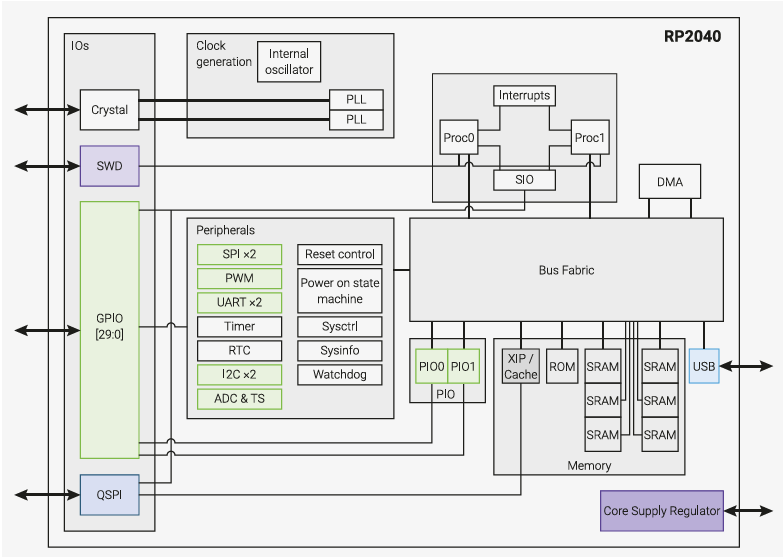
\includegraphics[width=0.6\textwidth]{rp2040_block_diagram.png}
        \caption{RP2040}
        \label{fig:RP2040}
    \end{figure}

    \item Przetwornika analogowo-cyfrowego 
    \begin{figure}[H]
        \centering
        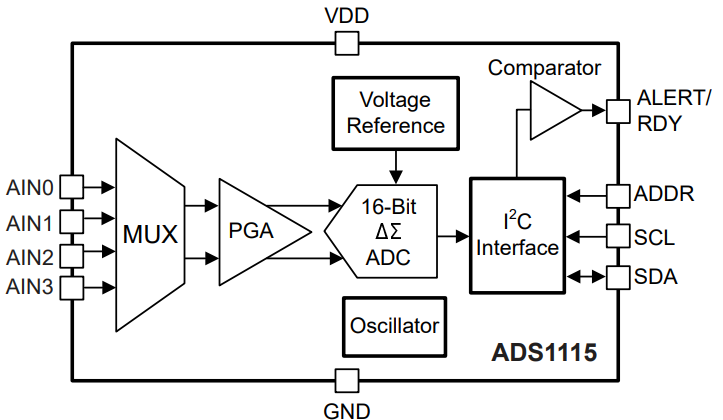
\includegraphics[width=0.6\textwidth]{ADC_block_diagram.png}
        \caption{ADS1115}
        \label{fig:ADS1115}
    \end{figure}

Schemat blokowy analizatora przedstawiono poniżej.
\begin{figure}[!ht]
    \centering
    \begin{circuitikz}
        \draw
            (0, 0) node[draw, minimum width = 6cm, minimum height = 3cm, align=center](PICO){\LARGE{Raspberry PI}\\\ \\\large{PICO W}}
            (3, -5)node[draw, minimum width = 12cm, minimum height = 3cm, align=center](PINS){\LARGE{Pin header}}

            (0, 4) node[draw, minimum width = 2cm, minimum height = 2cm](LDO){\LARGE{LDO}}
            % (5, 2) node[draw, minimum width = 2cm, minimum height = 2cm](V_REF){\LARGE{$\text{V}_{\text{ref}}$}}
            (6.5, 4) node[draw, minimum width = 2cm, minimum height = 2cm](ADC){\LARGE{ADC}}
            (5, 0) node[draw, minimum width = 2cm, minimum height = 2cm](AAF_PICO){\LARGE{AAF}}
            (8, 0) node[draw, minimum width = 2cm, minimum height = 2cm](AAF_ADC){\LARGE{AAF}}


            (PICO.west) to[short, -o] ++(-2, 0) node[above]{\large{USB}}
            (PICO.south) to[tmultiwire, l2=digital and logic, a=16] ++(0, -2)
            (LDO.south) to[short, a=$5V$] (PICO.north)

            (PICO.east) to[bmultiwire, l = 2] (AAF_PICO.west)
            (LDO) to[short, l=$3.3V$] (ADC) -| (8, 4) to[bmultiwire, l=2] (AAF_ADC.north)
            (ADC.south) --++ (0, -0.75) to[bmultiwire, a=$I^2C$] ++ (-5, 0) -- ++(0, -0.75)

            (AAF_PICO.south) to[bmultiwire, l=2] ++ (0, -2.5) 
            (AAF_ADC.south)  to[bmultiwire, l=2] ++ (0, -2.5)
        ;
    \end{circuitikz}
    \caption{Schemat blokowy analizatora stanów logicznych}
    \label{figure:block_diagram}
\end{figure}
\end{enumerate}

\useNormalLandscape{}
\subsection{Schemat ideowy analizatora}
    \begin{figure}[!ht]
        \centering
        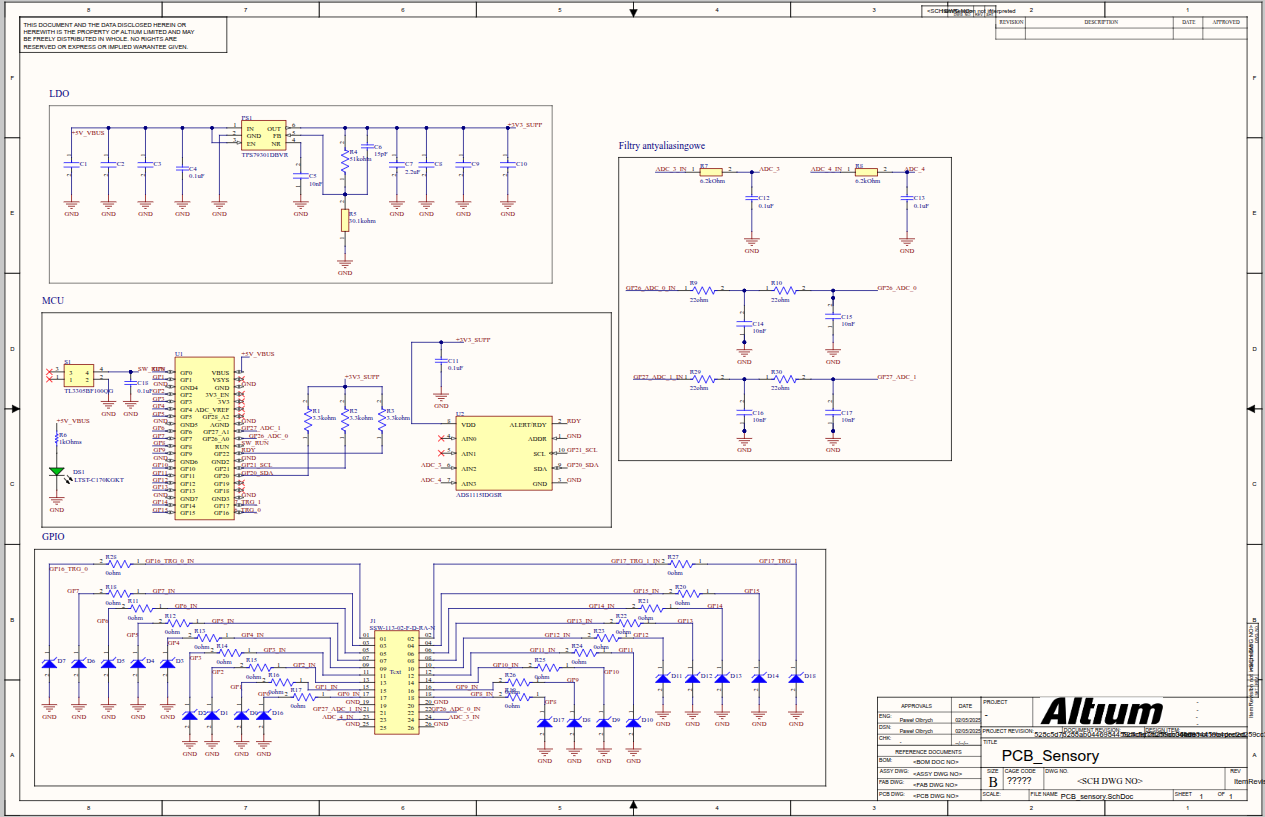
\includegraphics[width = 0.9\textwidth]{schematic.png}
        \caption{Schemat ideowy analizatora stanów logicznych}
    \end{figure}
\usePortrait{}

    W schemacie aplikacji do zabezpiecznia stopnia wejściowego analizatora dodano możliwość wlutowania rezystora ograniczająceg
    prąd wejściowy oraz zastosowano szybkie diody Zenera na 3.6V chronic go przed przepięciam napięciowymi. Układ taki działa
    również jako dolnoprzepustowy filtr RC, a z uwagi na małą pojemność diody (400pF), nie tłumi on sygnałów cyfrowych w paśmie
    pracy analizatora. Z kolei dla stabilnej pracy LDO oraz filtracji zakłóceń wysokoczęstotliwościowych, oprócz rekomendacji
    noty katalogowej, dodano po 3 kondensatory decaplingujace (3.3uF) na wejście oraz wyjście układu. 


\subsection{Opis płytki PCB}

    Płytka PCB analizatora stanów logicznych o wymiarach 74.3mm x 59mm została zaprojektowana w oprogramowaniu Altium Designer.
    Do poprowadzenia sygnałów miedzy blokami funkcyjnymi wykorzystano ścieżki na warstwie 1 i 4 o szerokości 10mil (0.254mm)
    oraz przelotki o wymiarach 0.3mm/0.6mm (otwór/średnica padu). 
    W celu zapewnienia jednoczesnego próbkowania sygnałów wejściowych w analizatorze stanów logicznych, starano zachować się
    jednakowe długości ścieżek sygnałowych prowadzących do wejść mikrokontrolera wykorzystując tzw. meandrowanie.
    Podejście takie było uwarunkowane tym, że różnice długości ścieżek sygnałowych prowadzą do zmian w czasie propagacji
    sygnału, co może powodować błędne rozpoznanie stanów logicznych lub zakłócenia synchronizacji danych. Zmontowane PCB
    wraz z przed przedstawiono na rysunku \ref{fig:PCB}. Dla układu zaprjektowano też specjalne podstawki chroniące przde zwarciem
    poprze położeniem na metalowych elemetnach.
    
\begin{figure}[H]
        \centering
        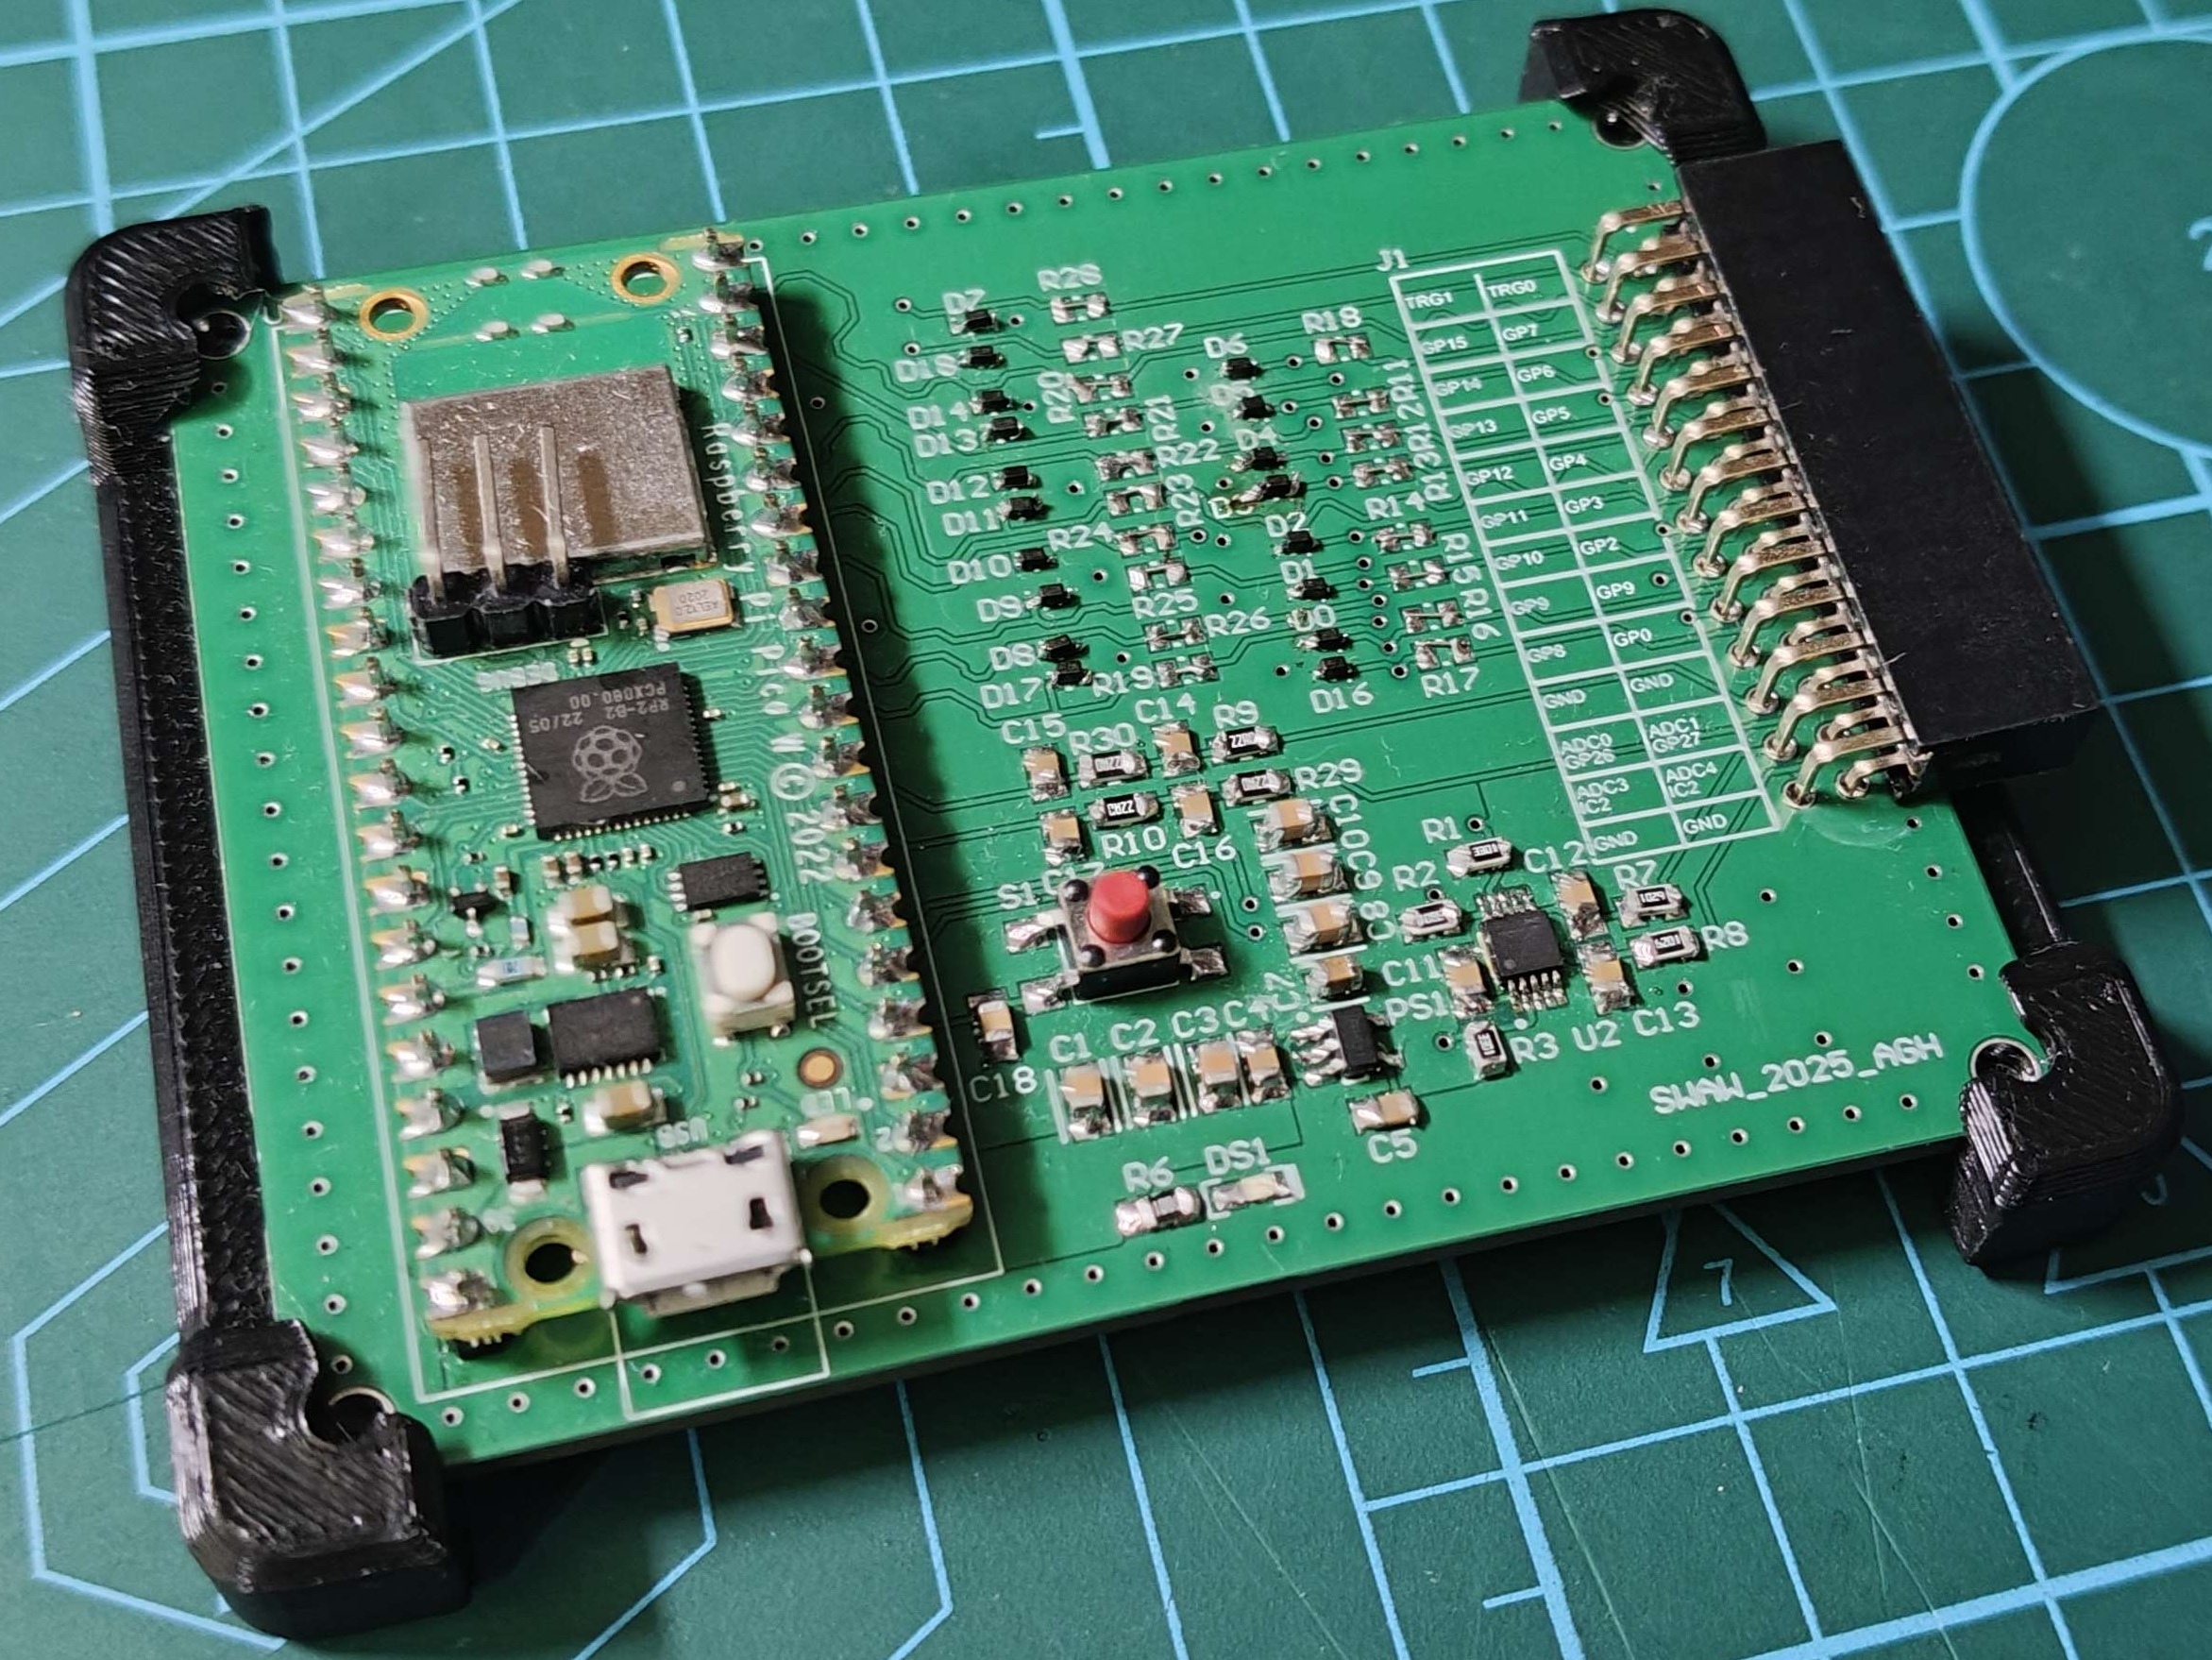
\includegraphics[width = 0.8\textwidth]{PCB.jpg}
        \caption{Widok zmontowanego PCB}
        \label{fig:PCB}
    \end{figure}

    \begin{figure}[H]
        \centering
        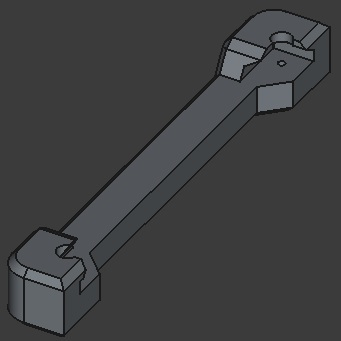
\includegraphics[width = 0.8\textwidth]{podstawka.jpg}
        \caption{Podstawka z druku 3D}
        \label{fig:podstawka}
    \end{figure}
    
    
\subsection{Stackup}
    Na rysunku \ref{fig:stackup}, przedstawiono wybrany stackup PCB proponowany przez firmę JLC PCB do projektów 4-o warstwowych.
    Zaletą jego stosowania jest GND na 2 oraz 3 warstwie poprawiajaca ciągłość masy ukałdu oraz skracająca pętle
    prądów powrotnych. Dodatkowo, taki wybór stackaup ogranicza przesłuchy i odbicia pomiędzy dolną i górną warstwą sygnałową
    czyniąc go dobrym wyborem dla naszej aplikacji. Widok w formacie gerber warsty 1 oraz 4 przedstawiono.
    na rysunku \ref{fig:gerber_top} i \ref{fig:gerber_bottom}. 
    \begin{figure}[H]
        \centering
        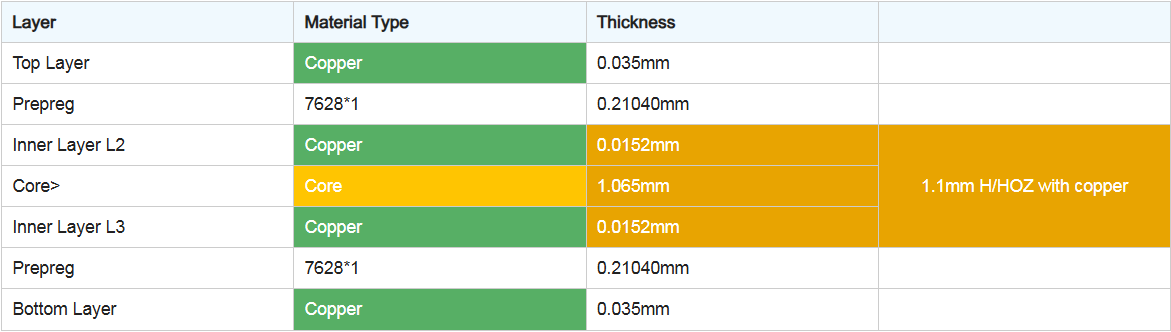
\includegraphics[width = 0.8\textwidth]{stackup.png}
        \caption{Stackup zalecany przez firmę JLC PCB}
        \label{fig:stackup}
    \end{figure}

    \begin{figure}[H]
        \centering
        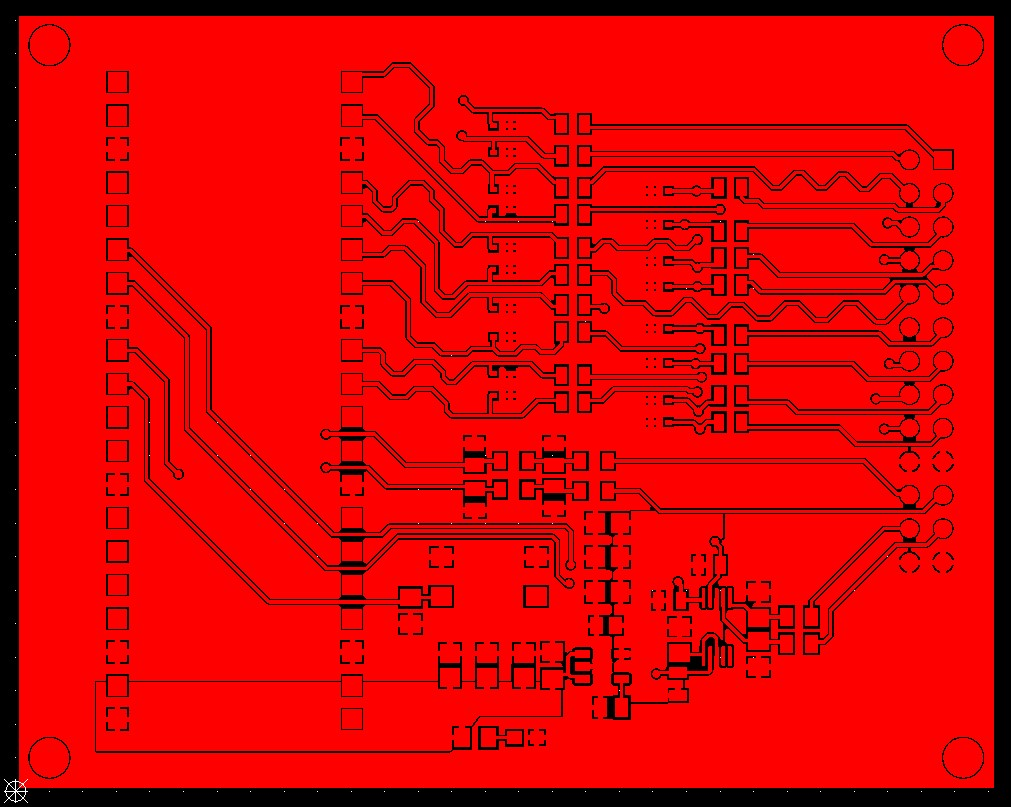
\includegraphics[width = 0.8\textwidth]{gerber_top.jpg}
        \caption{Widok pliku gerber warstwy 1 }
        \label{fig:gerber_top}
    \end{figure}

    \begin{figure}[H]
        \centering
        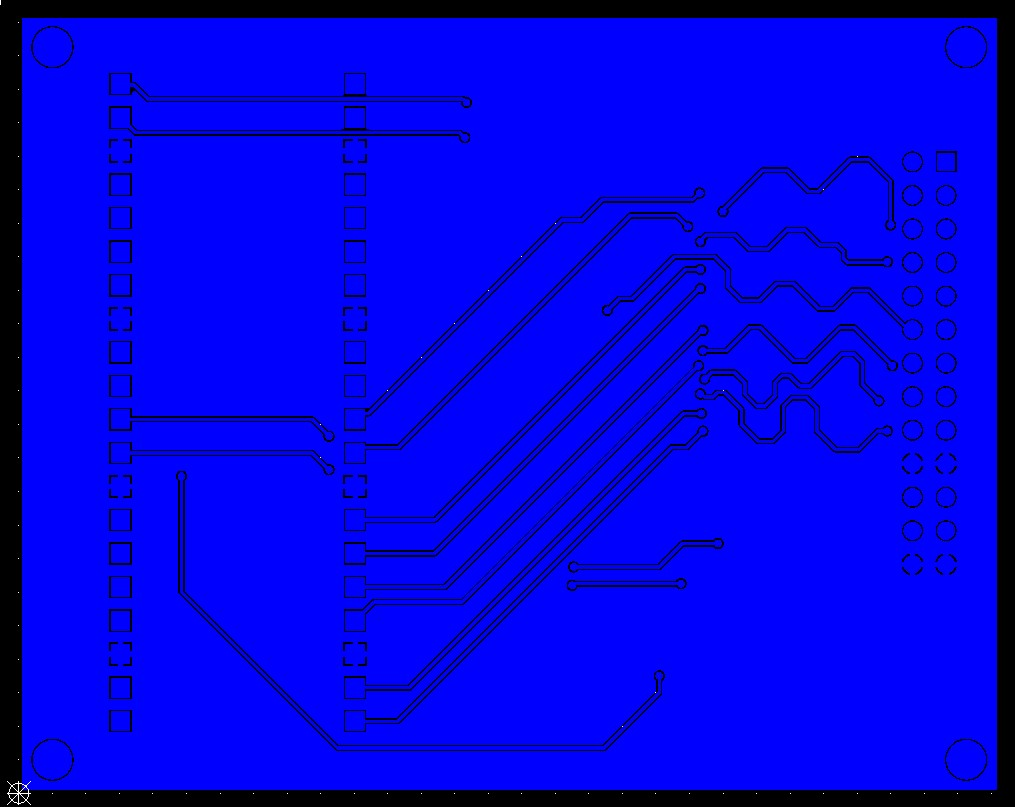
\includegraphics[width = 0.8\textwidth]{gerber_bottom.jpg}
        \caption{Widok pliku gerber warstwy 4 }
        \label{fig:gerber_bottom}
    \end{figure}

\subsection{Symulacje filtrów wejściowych}
Poniżej przedstawiono charakterystyki filtrów wejściowych sekcji analogowej.
\begin{figure}[!ht]
    \centering
    \begin{tikzpicture}
        \begin{axis}[
            width = 0.45\textwidth,
            grid = both,
            % axis lines= middle,
            % axis line style={->},
            xmin = 1, xmax = 10e3,
            xmode=log,
            title= Filtr ADS1115,
            ylabel = wzmocnienie ${[dB]}$,
            xlabel = częstotliwość ${[log(Hz)]}$
        ]
            \addplot table [x = freq, y =voltage, col sep = comma]{Measure/filter_ADS1115.csv};
            % \addplot table [x = duty, y = speedL, col sep = comma]{Measure/speed.csv};
        \end{axis}
    \end{tikzpicture}
    \begin{tikzpicture}
        \begin{axis}[
            width = 0.45\textwidth,
            grid = both,
            % axis lines= middle,
            % axis line style={->},
            xmin = 1e4, xmax = 3e6,
            xmode=log,
            title= Filtr PICO,
            ylabel = wzmocnienie ${[dB]}$,
            xlabel = częstotliwość ${[log(Hz)]}$
        ]
            \addplot table [x = freq, y =voltage, col sep = comma]{Measure/filter_PICO.csv};
            % \addplot table [x = duty, y = speedL, col sep = comma]{Measure/speed.csv};
        \end{axis}
    \end{tikzpicture}
    \caption{Wykresy tłumienia filtrów wejściowych}
\end{figure}
    \section{Analiza sygnałów logicznych}
    Analizator stanów cyfrowych w całości oparty jest na peryferiach wbudowanych w mikrokontroler.
    Jego najważniejszą część stanowi akcelerator IO, będący niewielką hardwarową maszyną stanów, 
    która umożliwia niezależnie od rdzeni wykonywać instrukcje sterujące portem wejścia-wyjścia,
    co w połączeniu z układami DMA, pozwala na pewną autonomię działania analizatora stanów logicznych.


\subsection{Implementacja analizatora stanów}
    Na rysunku \ref{fig:logic_stateMachine}, przedstawiono budowę automatu próbkującego dla sygnałów cyfrowych.

    \begin{figure}[!ht]
    \centering
    \begin{circuitikz}
        \draw
            (0,  0) node[draw, circle, align=center, minimum width = 3cm](trig){Oczekiwanie\\ na wyzwolenie}
            (4, -4) node[draw, circle, align=center, minimum width = 3cm](sample){Zebranie\\próbki}
            (0, -8) node[draw, circle, align=center, minimum width = 3cm](lock){Blokada\\wyzwalania}
            (8, -8) node[draw, circle, align=center, minimum width = 3cm](dma){Wyzwolenie\\DMA}
            (6, -12) node[draw, circle, align=center, minimum width = 3cm, dashed](time){Zapisanie\\czasu}
            (0, -12) node[draw, circle, align=center, minimum width = 3cm](store){Zapisanie\\próbki}
        ;

        \draw[very thick, -Stealth] (trig) to[bend left] node[right]{$trigger = 1$} (sample);
        \draw[very thick, -Stealth] (trig) to[loop left] (trig);
        \draw[very thick, -Stealth] (sample) to[bend left] (lock);
        \draw[very thick, -Stealth] (lock) to[bend left] node[left]{$trigger = 0$} (trig);

        \draw[very thick, -Stealth] (sample) to[bend right] (dma);
        \draw[very thick, -Stealth] (dma) to[bend left] (time);
        \draw[very thick, -Stealth] (time) to[short] (store);
    \end{circuitikz}
    \caption{Maszyna stanów, odpowiedzialna za akwizycję danych}
    \label{fig:logic_stateMachine}
\end{figure}

    Układ może być wyzwalany zewnętrzem sygnałem, przychodzącym na jedno z wejść cyfrowych lub na specjalnie wyznaczone wejście wyzwalające opisane jako $trig0$ lub $trig 1$.
    Alternatywnym sposobem wyzwalania próbkowania jest wykorzystanie wewnętrznego taktowania Raspberry PI PICO, dzięki czemu, można regularnie analizować stany z częstotliwością od $5kHz$ do maksymalnie $200MHz$.

    Dodatkową opcją, która może okazać się przydatna, jest pomiar czasu pomiędzy kolejnymi impulsami wyzwalającymi.
    Wykorzystuje ona jeden z kanałów PWM, jako licznik zliczający impulsy zegara - co pozwala mierzyć czas z maksymalną precyzją na poziomie $5ns$.
    Mechanizm ten wykorzystuje priorytetyzację modułów DMA, przez co maksymalna częstotliwość próbkowania spada do $50MHz$.


\subsection{Buforowanie w pamięci - synchronizacja DMA}
    Moduł analizatora wykorzystuje łącznie 4 z 12 dostępnych kanałów DMA, po dwa na zapisywanie próbek logicznych i dwa na zapisywanie czasu.
    Każda z par połączona jest w topologii typu ,,\textit{Ping-Pong}" dzięki czemu, kiedy jeden kanał zapełni się, natychmiast uruchamiany jest jego odpowiednik.
    Takie połączenie, umożliwia ciągłą (pierścieniową) praca układu próbkującego.

    Wszystkie cztery kanały wyzwalane są tym samym żądaniem ,,\textit{data request (DREQ)}".
    Wadą takiego rozwiązania jest synchronizacja procesu.
    Ponieważ zgłoszenie ,,\textit{DREQ}" jest rozgłoszeniowe, co w domyślnej konfiguracji, uniemożliwia określenie, która para zostanie wywołana jako pierwsza, przez co  może to powodować błędy zapisu czasu.
    Rozwiązaniem jest jawne nadanie wyższego priorytetu, dla pary obsługującej licznik.
    Poniżej przedstawiono graf pracy układów DMA w wyżej opisanym trybie.
    \begin{figure}[!ht]
    \centering
    \begin{circuitikz}
        \draw
            ( 0, 0) node[draw, circle, align=center, minimum width=3cm](dreq){Wyzwolenie\\DMA}
            ( 4, 0) node[draw, circle, align=center, minimum width=3cm](time){Zapis\\czasu}
            ( 8, 0) node[draw, circle, align=center, minimum width=3cm](sample){Zapis\\danych}
            (12, 0) node[draw, circle, align=center, minimum width=3cm](end){Zdjęcie\\flagi\\,,\textit{DREQ}''}
        ;

        \draw[very thick, -Stealth] (dreq) -- (time);
        \draw[very thick, -Stealth] (time) -- (sample);
        \draw[very thick, -Stealth] (sample) -- (end);
    \end{circuitikz}
    \caption{Łańcuch wyzwoleń kanałów DMA}
    \label{fig:dma_routine}
\end{figure}
    



    % Co więcej kanały odpowiedzialne za zapisywanie czasu, 


    \section{Przetwornik analogowo-cyfrowy}
Analizator wykorzystuje dwa przetworniki ADC:
\begin{itemize}
    \item Wewnętrzny - przetwornik SAR (Successive Approximation) o parametrach
        \begin{itemize}
            \item Typ : SAR
            \item Wykonanie : jeden przetwornik z multipleksowanym wejściem (4 wejścia + wewnętrzny pomiar temperatury)
            \item $f_{s\ max}$ = 500 kHz (dla jednego kanału)
            \item Rozdzielczość : 12 bit (8.7 ENOB)
            \item Tryb pracy: pojedynczy (brak możliwości badania sygnałów różnicowych) 
            \item $V_{in\ max}$ = 3.3 V
        \end{itemize}
        
    \item Zewnętrzny - przetwornik $\Delta\Sigma$ (Delta Sigma) - układ ADC1115
        \begin{itemize}
            \item Typ : Sigma - Delta
            \item Wykonanie : jeden przetwornik z multipleksowanym wejściem (4 wejścia) 
            \item $f_{s\ max}$ = 860 Hz (dla jednego kanału)
            \item Rozdzielczość : 16 bit 
            \item Tryb pracy: pojedynczy / różnicowy
            \item $V_{in\ max}$ = $2.048V$ - z możliwości regulacji programowej
        \end{itemize}
\end{itemize}

\subsection{Wewnętrzny przetwornik ADC (SAR)}
\subsubsection{Konfiguracja.}
Przetwornik wewnętrzny skonfigurowano w następujący sposób:
    \begin{itemize}
        \item $f_{s}$ = 5 kHz (z racji wykorzystania dwóch kanałów: $f_{sch1}$ = 2.5 kHz, $f_{sch1}$ = 2.5 kHz)
        \item Wyzwalanie konwersji : wyzwalanie za pomocą timera. 
    \end{itemize}

\subsubsection{Zasada działania.}
    Wewnętrzny przetwornik działa w oparciu o dwa bufory, które na zmianę zapełnia danymi. Takie 
    działanie pozwala przetwarzać (np. wysłać) ostatnio zebrane dane które przez okres 
    zapełniania drugiego bufora nie będą nadpisywane.

    Wyzwalaniem przetwornika zajmuje się timer, który odpytuje go o nowe dane z zadaną częstotliwością.
    Działanie przetwornika można by w znacznym stopniu zoptymalizować przez skonfigurowanie go w trybie kołowym oraz wykorzystaniu DMA. 
    W takim przypadku przetwornik sam zbierałby dane ze swojego wejścia następnie przełączał na kolejne a to co zebrał zapisywał do dedykowanego rejestru z którego dane były by odbierane przez DMA.
    Zaprojektowana biblioteka do obsługi ADC uwzględnia taką możliwość jednak w aktualnej wersji analizatora jest ona wyłączona na rzecz odpytywania przetwornika z poziomu przerwania od timera. 
    Głównym powodem takiego wyboru jest fakt dostępności tylko jednego DMA (multipleksowanego na 12 kanałów) oraz priorytetowej roli części cyfrowej (analizatora stanów logicznych).


\subsection{Zewnętrzny przetwornik ADC(ADS1115)}
Przetwornik zewnętrzny skonfigurowano w następujący sposób:
\begin{itemize}
    \item $f_{s}$ = 860 Hz(z racji wykorzystania dwóch kanałów: $f_{sch1}$ = 430 Hz, $f_{sch1}$ = 430 Hz)
    \item Wyzwalanie konwersji : wyzwalanie za pomocą timera. 
    \item Komunikacja : I2C (prędkość: 400kHz)
\end{itemize}

Zewnętrzny przetwornik podobnie jak ten dostępny w RP2040 również został skonfigurowany do cyklicznego odpytywania o nowe dane przez licznik (timer) oraz podobnie jak poprzednio jego praca opiera się o naprzemienne zapełnianie dwóch buforów (tym razem buforów kołowych). \\
Do komunikacji z mikrokontrolerem, ADS1115 wykorzystuje interfejs I2C skonfigurowany z prędkością 400 kHz.

\begin{figure}[ht]
    \centering
    \begin{tikzpicture}[
      buffer/.style={rectangle, draw, minimum width=2.5cm, minimum height=1cm, text centered},
      arrow/.style={-Stealth, thick},
      every node/.style={font=\small}
    ]
    
    % ADC
    \node[buffer, fill=blue!10] (adc) {ADC};
    
    % Buffers
    \node[buffer, fill=yellow!30, right=3cm of adc] (bufA) {Bufor A};
    \node[buffer, fill=orange!30, below=2cm of bufA] (bufB) {Bufor B};
    
    % Arrows from ADC
    \draw[arrow] (adc) -- node[above] {Próbkowanie} (bufA);
    
    % Processing
    \node[buffer, fill=green!20, right=2cm of bufA] (procA) {Przetwarzanie / Wysyłanie};
    
    \draw[arrow] (bufB) -- node[below, sloped] {wysyłanie} (procA);
    %\draw[arrow] (bufA) -- (procA);
    
    % Swapping arrows (loop)
    \draw[arrow, dashed] (bufA.south) to[bend right=20] node[left] {\shortstack{Zmiana\\buforów}} (bufB.north);
    \draw[arrow, dashed] (bufB.north) to[bend right=20] node[right] {} (bufA.south);
  
    \end{tikzpicture}
    \caption{Mechanizm podwójnego buforowania próbek z ADC}
    \label{fig:double-buffering}
  \end{figure}
    \section{Komunikacji analizatora z komputerem użytkownika}
Analizator do komunikacji wykorzystuje dwie metody transmisji: WIFI oraz USB.

\begin{figure}[ht]
    \centering
    \begin{tikzpicture}[
        device/.style={rectangle, draw, rounded corners, minimum width=4cm, minimum height=1.2cm, align=center, font=\small},
        arrow/.style={-Stealth, very thick},
        bidir/.style={Stealth-Stealth, thick, dashed}, % przerywana linia dwukierunkowa
        every node/.style={font=\small}
    ]

        % Komputer użytkownika
        \node[device, fill=blue!10] (pc) {Komputer użytkownika\\(dedykowana aplikacja)};

        % RP2040 jako AP
        \node[device, fill=green!20, right=6cm of pc] (pico) {RP2040 (Pico W)\\jako Access Point};

        \draw[bidir] (pc) -- ++(0,1) -- ++(10,0) -- ++(0,-0.4) node[below right, xshift=-6.5cm, yshift=1cm] {UDP przez Wi-Fi} (pico);
        \draw[-Stealth, Stealth-Stealth, very thick] (pc) -- ++(0,-1) -- ++(10,0) -- ++(0,0.4) node[below right, xshift=-6.5cm, yshift=-0.5cm] {Połączenie USB} (pico);

    \end{tikzpicture}
    \caption{Rozwiązanie kwestii transmisji w analizatorze}
    \label{fig:udp-komunikacja}
\end{figure}

\subsection{Komunikacja bezprzewodowa - WIFI}
    Do komunikacji bezprzewodowej wykorzystano układ CYW43439, dostępny na Raspberry PI Pico. 
    Jako protokół transmisyjny wykorzystano UDP ze względu na mały narzut
    obliczeniowy oraz mniejszą latencję, dodatkowo aby współpraca z urządzeniem była maksymalnie prosta ustawiono Pi Pico
    jako punkt dostępu (access point) oraz skonfigurowano na nim serwer DHCP który przydziela adresy
    IP podłączającym sie do niego użytkownikom. 

\subsection{Komunikacja przewodowa - USB}
    Układ RP2040 (jak i RP2350) wyposażone są w kontrolery $USB 1.2$ umożliwiające transmisję z maksymalną prędkością $12Mbps$,
    aby wykorzystać maksymalną przepustowość kanału, niezbędne jest stworzenie dodatkowego sterownika, po stronie odbiorcy.
    Aby maksymalnie uprościć proces przesyłania danych oraz zapewnić jak największą szybkość transmisji, kontroler USB został ustawiony w tryb CDC (Communication Device Class),
    pozwalający na emulację komunikacji szeregowej.

    Tak zaprogramowany mikrokontroler, pozwalana na prostą komunikację za pomocą portu szeregowego z szybkością nieporównywalną z klasycznymi układami \textit{USB UART}.\\
    W tabeli poniżej przedstawiono uśredniony czas wysłania wiadomości ,,Hello, world$\backslash$n$\backslash$r" w pętli 500 razy, za pomocą różnych rozwiązań:
    \begin{table}[!ht]
        \centering
        \caption{Średni czas wysłania wiadomości za pomocą różnych instrukcji}
        \begin{tabular}{|c|c|c|c|}\hline
            Protokół      & Polecenie wysłania & Zmierzony czas & Szybkość transmisji\\
            komunikacyjny & danych & $[ms]$& $[kbps]$\\\hline
            USB & tud\_cdc\_write &   1 520 & 294.74  \\\hline
            USB & printf          &   7 624 &  58.76  \\\hline
            UART& uart\_putc      & 604 732 &   0.74 \\\hline
            UART& printf          & 656 235 &   0.68 \\\hline
        \end{tabular}
    \end{table}

    Jak widać wykorzystanie sprzętowego kontrolera USB niesie ze sobą olbrzymią przewagę.
    Wyeliminowanie funkcji formatującej, pozwala przyspieszyć prędkość ponad pięciokrotnie!


\newpage
\subsection{Ramka transmisyjna}
    Powyższa analiza pozwoliła, zbudować warstwę fizyczną (\citetitle{Model_TCP_IP} \cite{Model_TCP_IP}).
    Następnym krokiem, powinna być (zgodnie z modelem TCP/IP) warstwa internetowa, jednak w przypadku sieci PAN, ten problemem rozwiązuje się samoistnie.
    Ostatnim krokiem poprzedzającym powstanie interfejsu użytkownika, zostaje zdefiniowanie ramki transmisyjnej.

    \subsubsection{Wielkość ramki danych}
        Wybór szerokości ramki, okazuje się nie trywialnym zadaniem i jest próbą znalezienia złotego środka między ograniczeniami sprzętowymi (pamięć RAM mikrokontrolera),
        czy wymogami standardów komunikacji (np. czas dostępu do okna transmisyjnego).

        W przypadku transmisji USB zgodnie z dokumentacją standardu \citetitle{USB20} \cite{USB20} maksymalna długość ramki jest ograniczona do 64 bajtów.
        Co oznacza, że wszystkie ramki dłuższe niż 64 bajty, będą przez kontroler USB rozdzielane na paczki po 64 bajty.
        Z tego względu, dobrym pomysłem wydaje się ramka o rozmiarze będącym całkowitą wielokrotnością 64.

        Inna sytuacja występuje podczas przesyłania danych bezprzewodowo.
        Ograniczeniem transmisji nie jest głębokość ramki (od 0 do nawet 2304 bajtów danych \citetitle{WiFi} \cite{WiFi}),
        natomiast synchroniczność przesyłania danych w ściśle określonych oknach czasowych.

        Podsumowując sensownym wydaję się ramka zawierająca między 64 a 512 bajtów.
    
    \subsection{Pola danych}
        Po określeniu rozmiaru transmisji, należy ustalić sposób ułożenia danych.
        Proponowane przez autorów rozwiązanie przedstawia rysunek \ref{fig:frame}.

        \begin{figure}[!ht]
            \centering
            \begin{circuitikz}
                \draw
                    (0, 0) node [draw, rectangle, minimum width = 2cm, minimum height = 2cm, align = center]{Tag\\2 bajty}
                    (2, 0) node [draw, rectangle, minimum width = 2cm, minimum height = 2cm, align = center]{Addition\\2 bajty}
                    (7, 0) node [draw, rectangle, minimum width = 8cm, minimum height = 2cm, align = center]{Payload\\60 - 508 bajtów}
                ;
            \end{circuitikz}
            \caption{Przykładowa ramka transmisyjna}
            \label{fig:frame}
        \end{figure}

        Opis pól w ramce:
        \begin{itemize}
            \item tag -- pole indetyfikacji, zawierające informację o tym co przenosi dana ramka,
            \item addition -- pole wypełniające, pole zawierające dwa zerowe bajty, możliwe do wykorzystania w przyszłości,
            \item payload -- pole z odpowiednimi danymi.
        \end{itemize}
    
    \subsection{Ułożenie danych}
        Moduł analizatora stanów logicznych w obecnej konfiguracji pozwala na dużą dowolność.
        Użytkownik może między innymi ustawić zapis próbek cyfrowych wraz z sygnaturą.
        Wymusza to jednak ograniczenia co do rozmiaru rozmiaru payload'u - jego głębokość musi być wielokrotnością 4 bajtów.
        Dzięki zastosowaniu tego ograniczenia, dane mogą być wysłane z przeplotem.

    \section{Interfejs graficzny}
    Aplikacja graficzna na komputery osobiste została napisana w języku \textit{C++} z wykorzystaniem biblioteki \textit{Qt}.
    Poniżej (rys. \ref{fig:gui}) przedstawiono poglądowe zdjęcie:

    \begin{figure}[!ht]
        \centering
        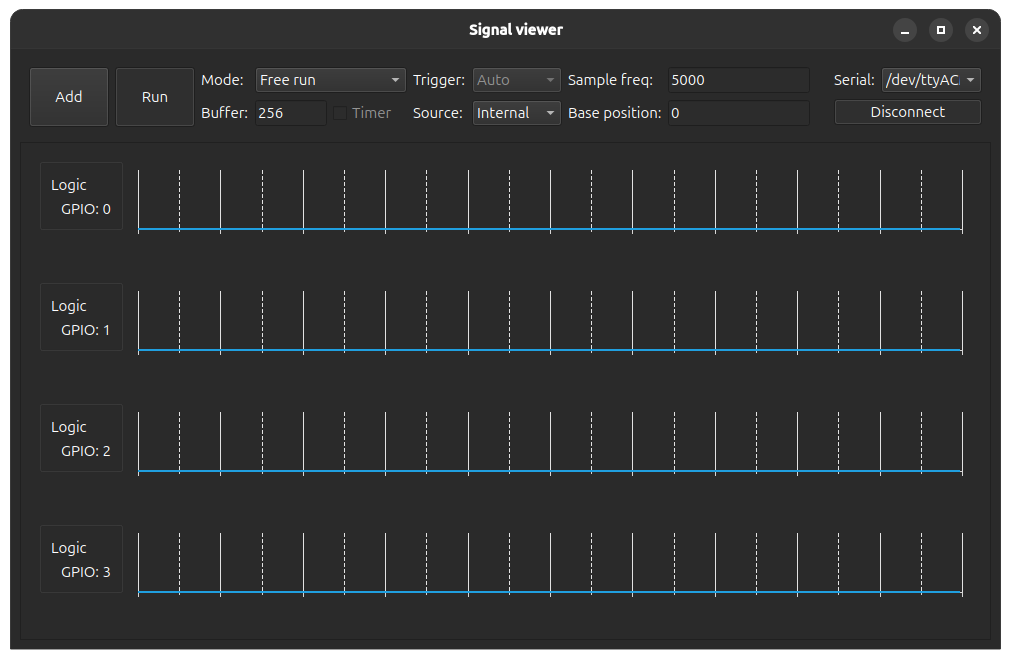
\includegraphics[width = 0.8\textwidth]{GUI.png}
        \caption{Zdjęcie aplikacji graficznej}
        \label{fig:gui}
    \end{figure}

    Dzięki wykorzystaniu biblioteki \textit{Qt}, aplikacja dynamicznie dostosowuje się do motywów systemowych co zaprezentowano na rysunku \ref{fig:gui_white}.
    \begin{figure}[!ht]
        \centering
        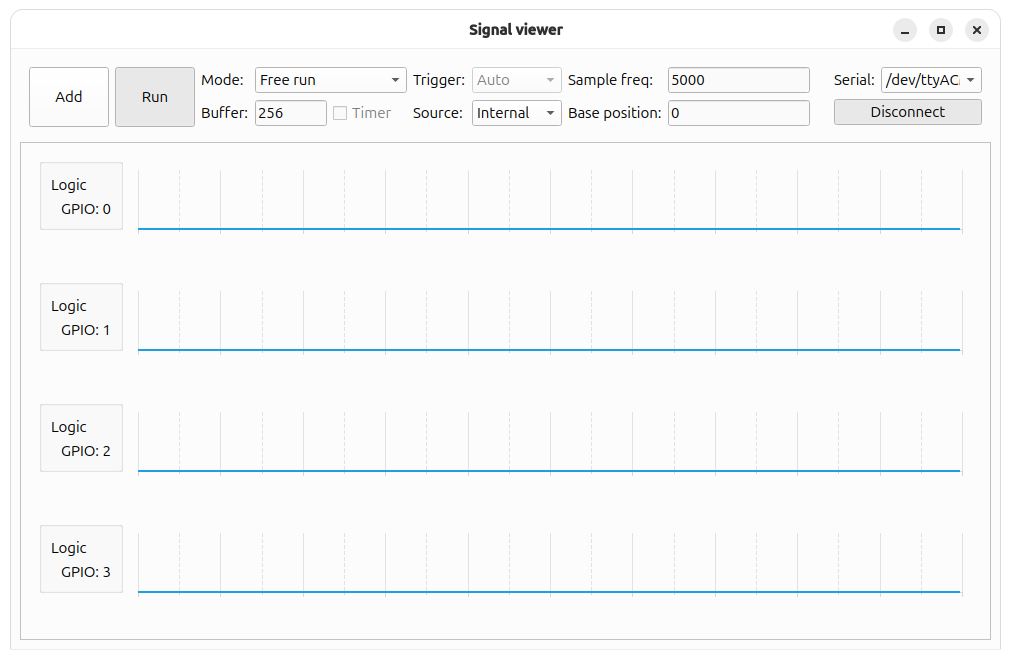
\includegraphics[width = 0.8\textwidth]{GUI_white.png}
        \caption{Zdjęcie aplikacji graficznej}
        \label{fig:gui_white}
    \end{figure}


    \subsection{Ustawienia analizatora}
        Z pomocą interfejsu użytkownika można zmieniać ustawienia analizatora stanów logicznych takie jak:
        \begin{enumerate}
            \item Tryb pracy analizatora:
            \begin{itemize}
                \item ,,Free run'' -- tryb pierścieniowy, po zapełnieniu całego bufora stare dane zostają nadpisane przez nowe,
                \item ,,Counted''  -- w tym trybie układ zbiera dokładnie określoną liczbę próbek zapisaną w polu \textit{Buffer}.
            \end{itemize}
            \item Źródło wyzwalania:
            \begin{itemize}
                \item Trigger   -- dwa dodatkowe wyprowadzenia służące wyłącznie do wyzwalania,
                \item GPIO      -- wyprowadzenia pomiarowe od 0 do 15,
                \item Internal  -- wyzwalanie wewnętrznym zegarem Raspberry PI PICO.
            \end{itemize}
            \item Częstotliwość próbkowania:
            \begin{itemize}
                \item w przypadku wyzwalania wewnętrznym zegarem to ustawienie odpowiada za częstotliwość wyzwalania,
                \item jeśli znacznik \textit{Timer} jest oznaczony, pole \textit{Sample freq.} odpowiada za częstotliwość pomiaru czasu.
            \end{itemize}
        \end{enumerate}

    \subsection{Wyświetlanie wykresów}
        W aplikacji można dynamicznie modyfikować liczbę wykresów.
        Po kliknięciu w przycisk ,,Add'' otwiera się dodatkowe okienko (rys. \ref{fig:gui_addPlot}) z poziomu,
        którego użytkownik może dodawać różnego rodzaju wykresy.
        \begin{figure}[!ht]
            \centering
            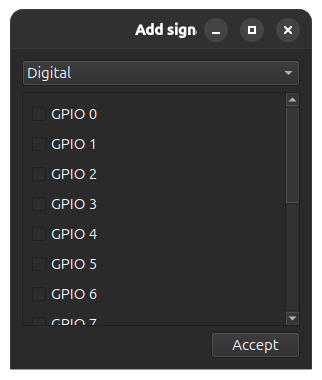
\includegraphics[width = 0.4\textwidth]{GUI_addPlot.png}
            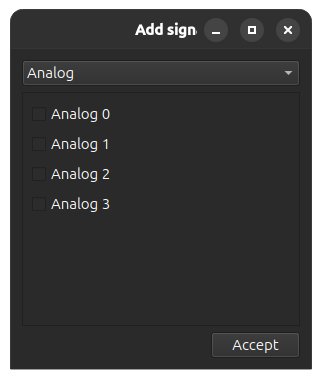
\includegraphics[width = 0.4\textwidth]{GUI_addAnalog.png}
            \caption{Okienko dodawania wykresów}
            \label{fig:gui_addPlot}
        \end{figure}

        Wykresy można także dynamicznie usuwać, po kliknięciu w niechciany wykres prawym przyciskiem myszy pojawia się rozwijane menu z opcją \textit{Remove}.
        Co zaprezentowano na rysunku poniżej.

        \begin{figure}[!ht]
            \centering
            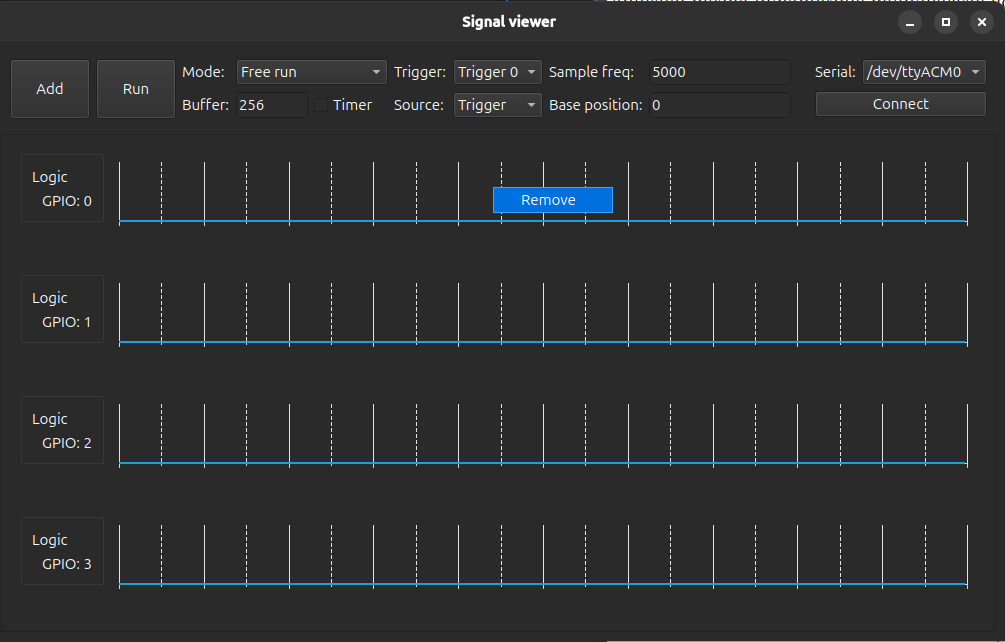
\includegraphics[width = 0.8\textwidth]{GUI_remove.png}
            \caption{Usuwanie pierwszego wykresu}
            \label{fig:gui_removePlot}
        \end{figure}

    
    \subsection{Pomiary}
        W celu rozpoczęcia pomiarów, należy podłączyć analizator do komputera, 
        następnie z listy rozsuwanej po prawej stonie wybrać port szeregowy,
        pod którym przedstawiło się urządzenie.

        W momencie podłączenia urządzenia do komputera zapala się zielona dioda na PCB informująca o zasilaniu układu a także
        druga zielona dioda LED tym razem dostępna na Raspberry Pi Pico, której miganie symbolizuje poprawny start analizatora oraz gotowość do rozpoczęcia pomiarów.
        Następnie po wybraniu trybu pracy i wciśnięciu przycisku \textit{RUN} w aplikacji graficznej, analizator rozpoczyna pracę,
        co sygnalizowane jest przez zatrzymanie się błyskającej diody.
    
    \subsection{Do dokończenia}
        Aktualna wersja aplikacji nie pozwala na komunikację sieciową, nie zawiera także implementacji wyświetlania sygnałów analogowych.

    \subsection{Błędy w kodzie}
        W obecnej wersji GUI jest możliwość wyboru trigger'a.
        Jednak ze względu na błąd w kodzie, analizator nie zmienia częstotliwości próbkowania, podczas wybrania wewnętrznego wyzwalania - ustawiona jest domyślna częstotliwość 5kHz.
        
        Dodatkowo, podczas analizy wyzwalanej zewnętrznym trigger'em aplikacja czasami zamyka się z błędem \textit{,,IOT instruction (core dumped)''}.
        Problem ten, nie występuje podczas pracy na wewnętrznym taktowaniu.

        Ostatnim zauważonym bugiem w aplikacji, jest niepoprawne czyszczenie bufora komunikacji przewodowej.
        Z jakiegoś powodu, czasem po próbie ponownego uruchomienia analizatora, ten nie reaguje na komendę startu.



    \section{Opis sposobu zarządzanie zadaniami w systemie dwurdzeniowym analizatora.}

Analizator stanów logicznych ze względu na bardzo rozbudowany system kontrolno-pomiarowy
został zaprojektowany tak aby podzielić konieczne do zrealizowania zadania na dwa dostępne w 
rp2040 rdzenie. \\
Rdzeń 0 jest głównym rdzeniem(masterem) który pełni nadrzędną rolę w sterowaniu całym urządzeniem,
natomiast rdzeń 1 pełni rolę podrzędną(slave'a) odpowiedzialnego za komunikację bezprzewodową oraz akwizycje danych analogowych.
Dokładny opis zadań realizowanych przez poszczególne rdzenie przedstawiono poniżej.

\begin{itemize}
    \item Rdzeń 0
    Rdzeń 0 (podstawowy rdzeń mikrokontrolera rp2040) odpowiedzialny jest min. za:
    \begin{itemize}
        \item Oczekiwanie na sygnał wyzwalający pomiar (trigger)
        \item Zapisanie czasu pomiędzy wystąpieniami sygnału trigger (opcjonalnie) 
        \item Zbieranie danych z wejść cyfrowych z wykorzystaniem DMA
        \item Wysyłanie zebranych danych pomiarowych przez interfejs USB do komputera użytkownika
    \end{itemize}

    \item Rdzeń 1
    Rdzeń 1 odpowiedzialny jest za:
    \begin{itemize}
        \item Próbkowanie sygnału z kanału 0 przetwornika ADC ADS1115
        \item Próbkowanie sygnału z kanału 1 przetwornika ADC ADS1115
        \item Próbkowanie sygnału z kanału 3 wbudowanego przetwornika ADC RP2040
        \item Próbkowanie sygnału z kanału 4 wbudowanego przetwornika ADC RP2040
        \item Wysyłanie zebranych danych przez WIFI do komputera użytkownika
        \item Wysyłanie zebranych danych pomiarowych do rdzenia 0
        \item Wysyłanie odebranych danych sterujących do rdzenia 0 (jeżeli takie odebrano)
        \item Odbieranie danych sterujących od aplikacji użytkownika
        \item Przydzielanie adresu IP użytkownikowi który połączy się z analizatorem 
    \end{itemize}

    \item Komunikacja między rdzeniem 0 i rdzeniem 1
    \begin{figure}[h!]
    \centering
    \begin{tikzpicture}[
        corebox/.style={
            rectangle,
            draw=blue!35!black,
            line width=1mm,
            fill=blue!10,
            rounded corners,
            minimum width=7cm,
            minimum height=10cm,
            align=left,
            text width=6cm,
            font=\bfseries
        },
        arrow/.style={
            <->,
            ultra thick,
            draw=blue!70!black
        }
    ]

    % Box for Core 0
    \node[corebox, label=above:{\textbf{Rdzeń 0}}] (core0) {
        \begin{enumerate}
            \item Czekaj na sygnał wyzwalający (trigger)
            \item Zapisz czas między wystąpieniami sygnału trigger (opcjonalnie) 
            \item Zbierz dane z wejść cyfrowych z wykorzystaniem DMA
            \item Wysyślij zebrane dane przez interfejs USB do komputera użytkownika
        \end{enumerate}
    };

    % Box for Core 1
    \node[corebox, right=3cm of core0, label=above:{\textbf{Rdzeń 1}}] (core1) {
        \begin{enumerate}
            \item Zbierz dane z przetworników ADS1115 oraz Pico ADC
            \item Wyślij zebrane dane przez Wi-Fi do komputera użytkownika
            \item Wyślij zebrane dane do rdzenia 0
            \item Odbierz dane sterujące(jeżeli take są)
            \item Przydziel adres IP użytkownikowi
        \end{enumerate}
    };

    % Arrow between cores
    \draw[arrow] (core0.east) -- node[above, font=\bfseries] {FIFO} (core1.west);

    \end{tikzpicture}
    \caption{Podział zadań między rdzeniami mikrokontrolera}
\end{figure}


\end{itemize}


    \section{Analizator sygnałów analogowych - test zaprojektowanego systemu.}
    Kolejnym etapem projektowania układu do pomiaru sygnałów analogowych było przetestowanie 
    zaprojektowanego systemu.

\subsection{Opis stanowiska pomiarowego.}
    Pomiary wykonano z użyciem generatora \textit{DDS FG-100 DDS FUNCTION GENERATOR}
    oraz przenośnego oscyloskopu \textit{Fnirsi 1c15} jako układu odniesienia z pomocą którego
    zadawano parametry generowanych sygnałów. Stanowisko pomiarowe przedstawiono poniżej.

    \begin{figure}[!ht]
        \centering
        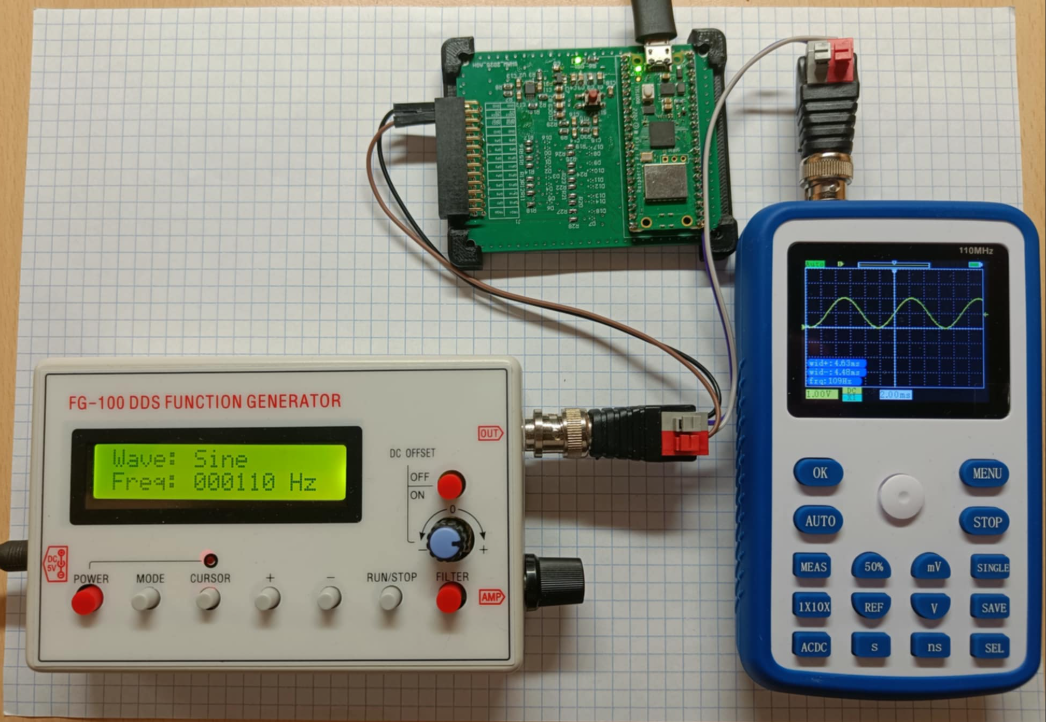
\includegraphics[width = \textwidth]{stanowisko_pomiarowe.png}
        \caption{Układ stanowiska pomiarowego}
        \label{fig:stanowisko_pomiarowe}
    \end{figure} 

    W celu przeprowadzeniu testów działania systemu, które na wczesnym etapie projektu
    mogłyby się odbywać niezależnie od aplikacji graficznej, postanowiono napisać
    skrypt w języku Python, dzieki któremu możliwe było obserwowanie zebranych danych
    wysyłanych przez WIFI do komputera. Widok aplikacji przedstawiono poniżej.
    
    \begin{figure}[H]
        \centering
        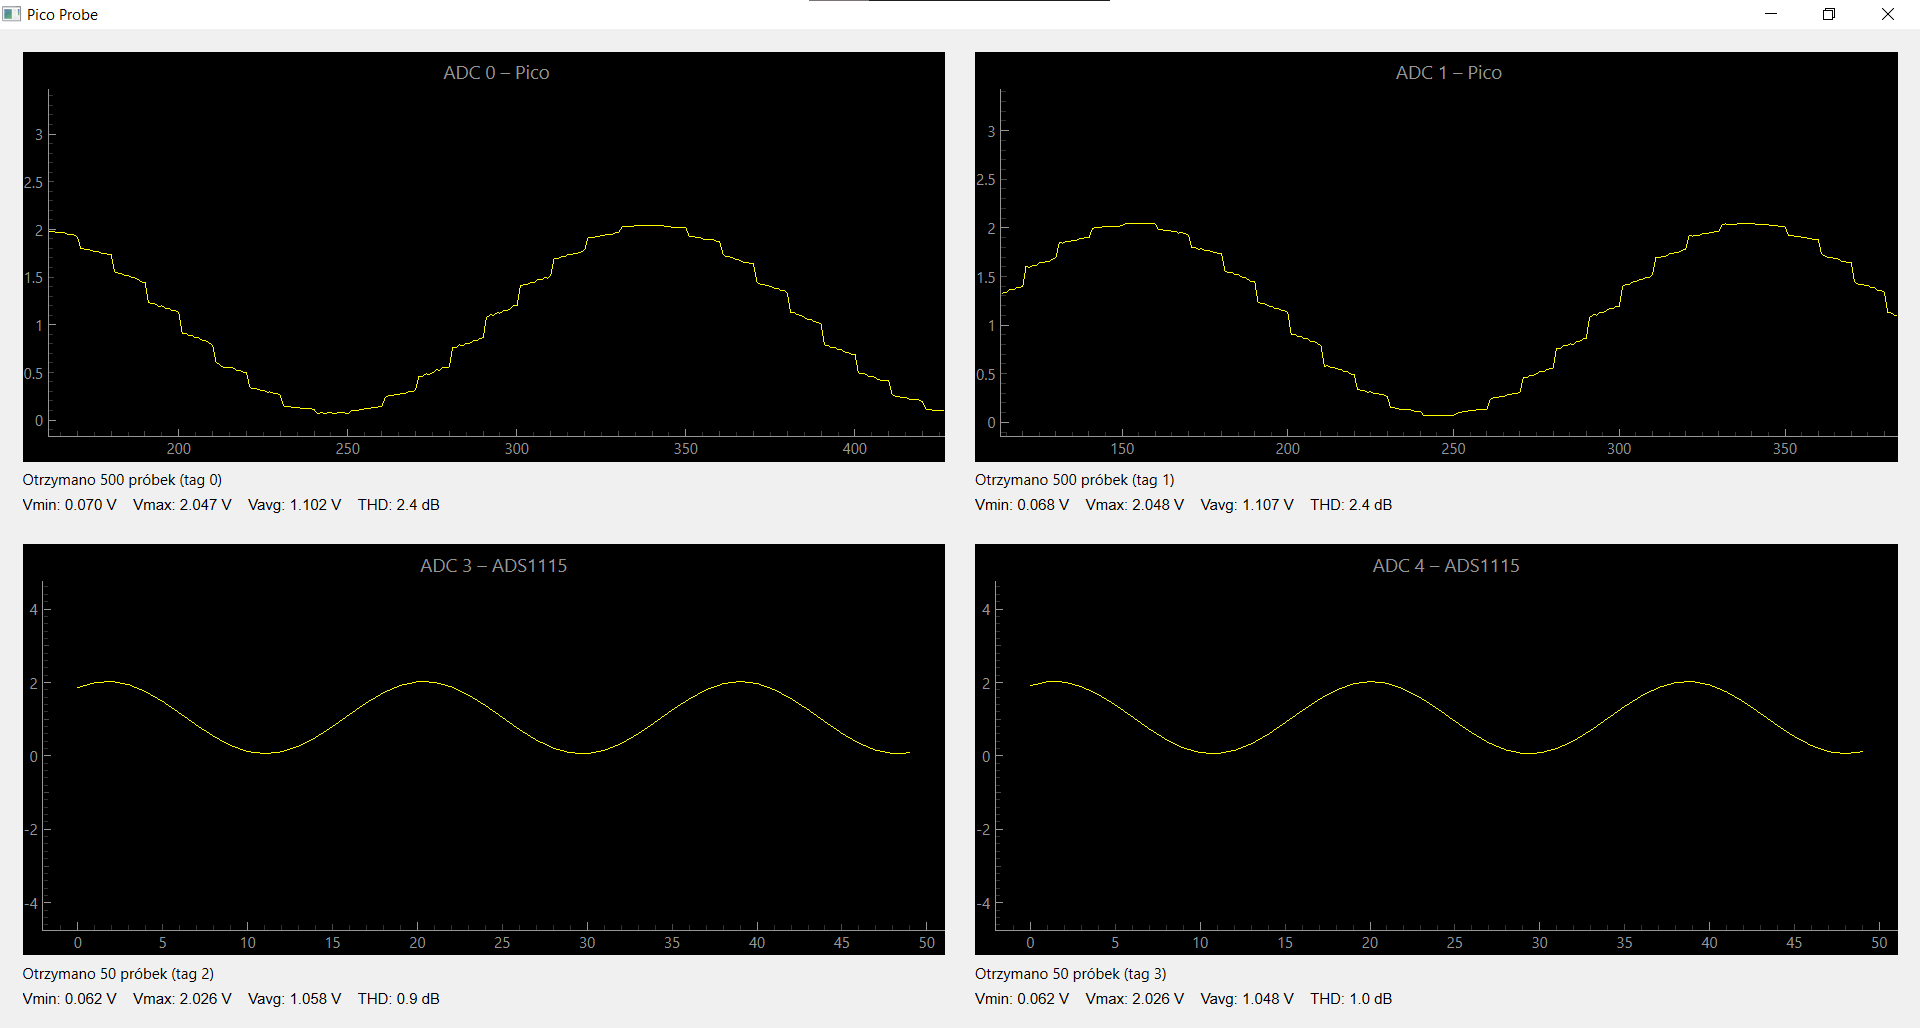
\includegraphics[width = \textwidth]{Analog_track_2.png}
        \caption{Pomocnicza aplikacja do obserwowania przebiegów sygnałów analogowych}
        \label{fig:Analog_track_2}
    \end{figure}

\subsection{Testowanie działania analizatora sygnałów analogowych}
    Jednym z najważniejszych parametrów przy testowaniu układów takich jak oscyloskopy
    czy ogólnie analizatory sygnałów analogowych jest min. maksymalna częstotliwość
    sygnałów które wiernie mogą odwzorowywać. Częstotliwość ta wynika bezpośrednio z 
    twierdzenia o próbkowaniu Nyquista-Shannona:
    \[
    f_s \geq 2 f_{\max}
    \]

    W rzeczywistości jednak częstotliwość próbkowania powinna być większa niż 
    dwukrotność maksymalnej składowej częstotliwościowej sygnału, często podaje się ją
    jako:
    \[
    f_s \geq 2.5 f_{\max}
    \]
    lub nawet więcej.

    Podczas przeprowadzenia testów, kryterium badania jakości mierzonych sygnałów była wartość
    THD(dla 4 harmonicznych), którą definiuje się następująco:
    \[
    \mathrm{THD}_{dB} = 20 \log_{10} \left( \frac{
    \sqrt{
    \sum_{h=2}^{5} \left|X(h f_1)\right|^2
    }
    }{
    \left|X(f_1)\right|
    } \right)
    \]
    Jeżeli więc zniekształcenia osiągały duże wartości(małe THD, czyli dużą zawartość
    pozostałych harmonicznych względem podstawowej) stwierdzano, że dalsze zwiększanie częstotliwości nie ma sensu
    i kończono pomiar na niej. Zebrane wyniki pomiarów przedstawiono poniżej.

    \begin{table}[!ht]
        \centering
        \begin{tabular}{|c|>{\centering\arraybackslash}m{4cm}|>{\centering\arraybackslash}m{4cm}|}
            \hline
            \textbf{Nazwa przetwornika} &
            \makecell{\textbf{Teoretyczna maks.}\\\textbf{częstotliwość}} &
            \makecell{\textbf{Zmierzona maks.}\\\textbf{częstotliwość}} \\
            \hline
            ADS1115 & 250 Hz & 180 Hz \\
            \hline
            Pico ADC & 2.5 kHz & 250 Hz \\
            \hline
        \end{tabular}
        \caption{Wyniki testów analizatora sygnałów analogowych}
        \label{tab:freq_test_results}
    \end{table}

    \subsection{Zaobserwowane problemy z działaniem układu.}
    Jak można było to już wcześniej zauważyć(rys.~\ref{fig:Analog_track_2})
    wykres amplitudowy z ADC Pico jest mocno zniekształcony, jeszcze lepiej
    widać to na poniższej ilustracji.
     
    \begin{figure}[H]
        \centering
        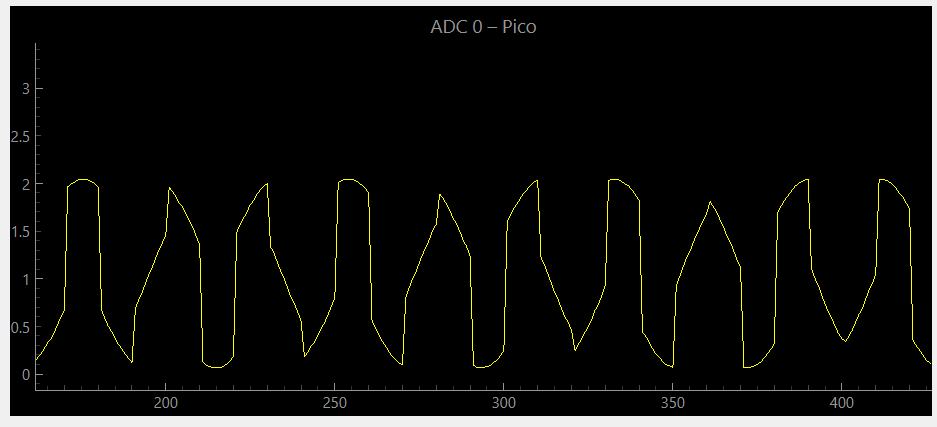
\includegraphics[width = \textwidth]{analog_distortion.png}
        \caption{Wstępnie przetworzony sygnał wyjściowy z ADC Pico}
        \label{fig:analog_distortion}
    \end{figure}

    Charakter wykresu nie jest spowodowany zbyt wysoką częstotliwością podawanego
    sygnału lecz skutkiem działania systemu. Duże zniekształcenia sygnału wynikają
    z transmisji I2C która z racji na bardzo sprzętowy charakter, jeżeli wystąpi blokuje
    cały rdzeń w skutek, czego to co zbiera ADC Pico jest mocno zniekształcone.
    Podczas projektowania układu podejmowano różne techniki niwelowania takiego zachowania tj.: 
    \begin{enumerate}
        \item Praca z I2C na przerwaniach z wykorzystaniem maszyny stanów.
        \item Wykorzystanie wbudowanej funkcjonalności ADS1115 która umożliwia zgłaszanie przez.
        przetwornik zdarzenia zakończenia konwersji przez co nie trzeba na nią czekać tracąc czas
        rdzenia.
    \end{enumerate}

    Innym pomysłem na rozwiązanie tego problemu było by zastosowanie innego przetwornika ADC wykorzystującego szybsze protokoły transmisji(np. SPI)
    lub inne topologie wewnętrznego ADC.

    Niestety ostatecznie nie udało się doprowadzić żadnej z wyżej wymienionych opcji do stanu
    który można by uznać za zadowalający, głównie ze względu na rosnącą złożoność sytemu kontrolno-pomiarowego
    którego dobrze działająca implementacja okazała się bardzo pracochłonna i skomplikowana.
    
    Dlatego właśnie maksymalna częstotliwość Pico ADC pomimo znacznie większego
    próbkowania ostatecznie okazała się niedużo większa niż znacznie wolniejszego ADS1115.  
    \section{Analizator sygnałów logicznych - test zaprojektowanego systemu}
    W celu przetestowania układu należy wygenerować odpowiednio duży wektor testowy,
    pozwalający na rzetelne sprawdzenie wszystkich możliwych kombinacji.
    Jednocześnie wektor ten powinien był w miarę możliwości prosty do sprawdzenia.
    Dlatego też jako wektor testowy wykorzystano licznik binarny, który z każdym stanem powinien rosnąć o dokładnie \textit{,,1''}.

    Poniżej przedstawiono zdjęcie aplikacji wyświetlającej 512 próbek odebranych za pomocą analizatora.
    \begin{figure}[!ht]
        \centering
        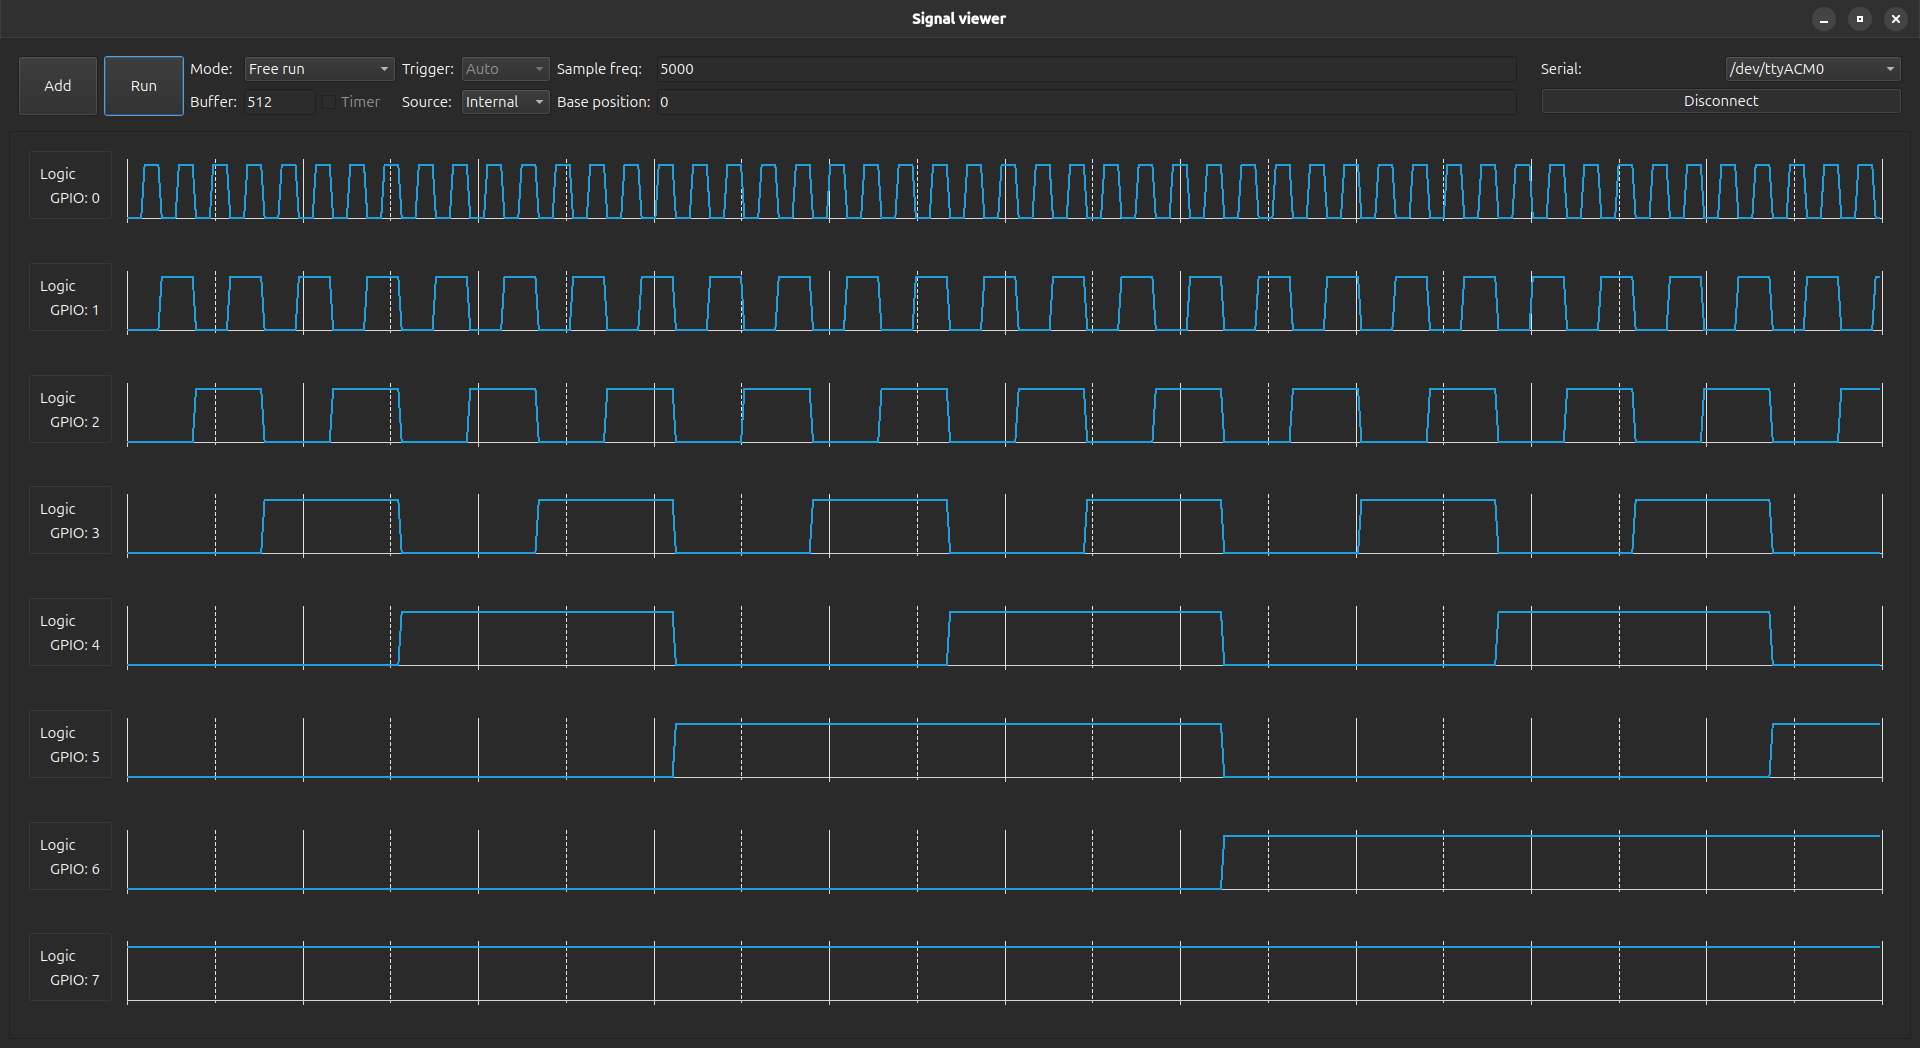
\includegraphics[width=0.8\textwidth]{test_1khz.png}
        \caption{Zdjęcie aplikacji - pomiar testowy, częstotliwość sygnału 1kHz}
    \end{figure}

    Odczytana częstotliwość na podstawie ilości próbek: $f_{read} = 1kHz$, co odpowiada zadanej częstotliwości wejściowej.

    Analizowanie wyższych częstotliwości w aktualnej wersji programu graficznego jest niemożliwe, ze względu na bug w kodzie aplikacji, która nie zmienia ustawień analizatora.
    Natomiast przed rozpoczęciem pracy z aplikacją graficzną, analizator został przetestowany, sygnał cyfrowym przedstawionym poniżej:
    \begin{figure}[!ht]
        \centering
        \begin{tikzpicture}
            \draw
                (0, 0) 
                    --++ (1, 0) --++(0, 1) --++(1, 0) --++ (0, -1)
                    --++ (1, 0) --++(0, 1) --++(1, 0) --++ (0, -1)
                    --++ (1, 0) --++(0, 1) --++(1, 0) --++ (0, -1)
                    --++ (1, 0) --++(0, 1) --++(1, 0) --++ (0, -1)

                    --++(4, 0)
                    --++ (1, 0) --++(0, 1) --++(1, 0) --++ (0, -1)
            ;

            \draw [Stealth-Stealth] (2, 1.5) -- node[above]{50MHz} (4, 1.5);
            \draw [Stealth-Stealth] (1, -0.5) -- node[above]{1kHz} (13, -0.5);
        \end{tikzpicture}
    \end{figure}

    Dla takiego sygnału udało się odebrać odebrać licznik binarny, którego złożenie przedstawiono na wykresie \ref{fig:sampling}.
    \newpage
    \begin{figure}[!ht]
        \centering
        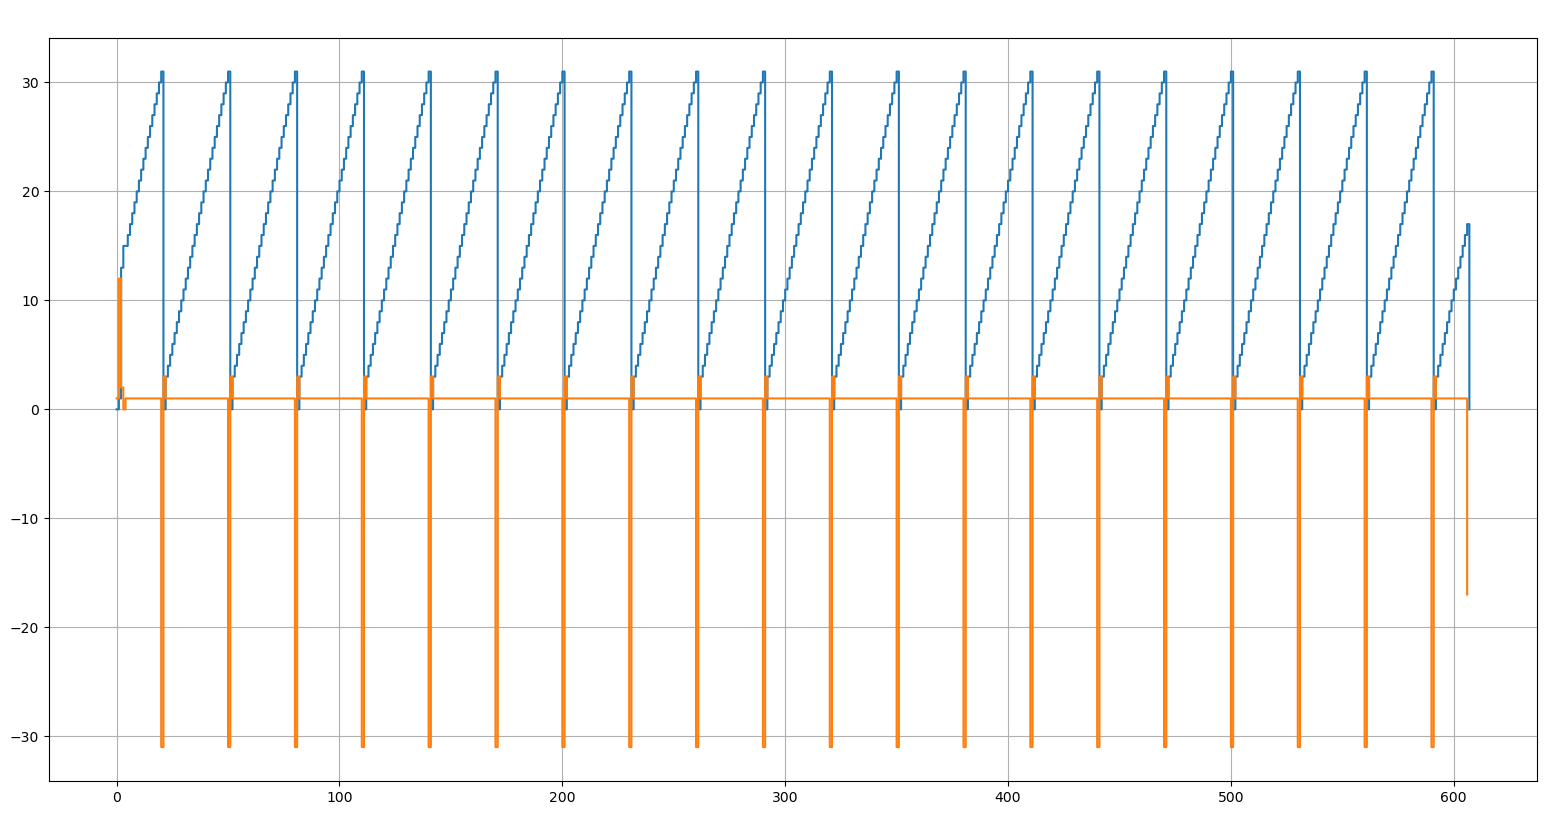
\includegraphics[width=0.8\textwidth]{Sampling.png}
        \caption{Wykres przebiegu odebranego dla sygnału o maksymalnej częstotliwości $50MHz$}
        \label{fig:sampling}
    \end{figure}
    \begin{itemize}
        \item na pomarańczowo oznaczono różnicę między aktualną a poprzednią próbką,
        \item niebieskim zaprezentowano odebraną próbkę.
    \end{itemize}

    \subsection{Zaobserwowane problemy z działaniem analizatora}
        Największym problemy działania analizatora jest utrata próbek podczas analizy bardzo szybkich sygnałów w trybie \textit{Free Run}.
        Podczas pracy kołowej kołowej analizator nie jest w stanie wysyłać próbek tak szybko jak układ PIO i DMA zapisują nowe dane.
        Rozwiązaniem tego problemu jest nie wykorzystywanie tego trybu do analizy ciągłych bardzo szybkich sygnałów.


    

    \vfill
    \begin{flushright}
        Łukasz Przystupa,\\
        Krzysztof Płonka,\\
        Paweł Olbrych
    \end{flushright}


    \newpage
    \pagenumbering{gobble}
    \nocite{*}
    \printbibliography
\end{document}
